\documentclass[a4paper,12pt]{report}

\usepackage[utf8]{inputenc}
\usepackage[T1]{fontenc}
\usepackage{array}
\usepackage{amsmath}
\usepackage[english]{babel}
\usepackage{bm}
\usepackage{graphicx}
\usepackage[a4paper]{geometry}
\usepackage[colorlinks=true,urlcolor=blue,linkcolor=blue]{hyperref}
\usepackage{url}
\usepackage[nottoc,numbib]{tocbibind}
\usepackage{color}
\usepackage{epstopdf}
\usepackage{xcolor}
\usepackage{rotating}
%\usepackage{wrapfig,booktabs}
\usepackage[backend=biber,style=phys]{biblatex}
\usepackage{upgreek}
\usepackage[capbesideposition={right,center}]{floatrow}

\addbibresource{../Bibliography.bib}

\makeatletter
	\renewcommand{\thechapter}{\Roman{chapter}}
\makeatother

\floatsetup[table]{style=plaintop}

\begin{document}

\chapter{Magneto-optical study of Cr-doped CdTe quantum dots\label{MagOptStud}}

%Plan:
%	Part I:
%		- On a vu du Cr. PL caractéristique en quatres pics, dont le second à plus haute énergie peut-être splitté. 
%		- Cr splitté par les contraintes bi-axiales. $S_z = \pm 2$ a assez haute énergie qu'ils ne peuvent pas être peuplé thermiquement. Raie splittée polaréisée linéairement correspond au 0.
%		- PL résolue en temps de la raie LE deux foiss plus longue que les autres -> peut correspondre à des dark exciton.
%		- Augmentation de la température -> pas d'apparition de $S_z = \pm 2$. De plus, $S_z = \pm 1$ disparaisse très rapidement => meilleure couplage aux noirs ?
%		- Bon couplage aux phonons optiques et accoustiques observé lors de la PLE.
%		- Etats avec une bonne conservation du spin observé dans la PLE.
%		- Magneto-optique confirme la structure énergétique. Plusieurs anti-crossing visible nous aide à identifier les états.
%		- La répartiton en intensité est compatible avec un couplage h-Cr anti-ferromaganétque. Cela peut-être du aux contrainted faisant bouger les niveaux du Cr et les bandes de CdTe.
%	Part II:
%		- Modèle de spin effectif prenant en compte la structure du Cr dans CdTe, l'interaction d'échange porteur-Cr et elecron-trou, l'effet Zeeman et le shift diamagnétique et le VBM reproduit bien effets observés expérimentalement. Une valeur de $D_0$ comprise entre 2 et 3 meV est déduite.
%		- Simulation de boîtes avec un fort E indique la possibilité d'observer de la polarisation linéaire sur toutes les raies. Pics peuvent ne pas être résolus -> pas trouvables pour nous (sélection de boîtes à faible E).
%	Part III:
%		- Boîtes trouvées présentant de la polar linéaire sur le trois raies. Mais magnéto-optique n'indique pas d'atome magnétique dedans. Evolution sous champs permets de changer le splitting.
%		- Hypothèse possible : Cr en dehors des boîtes. 3 états de charges possibles dans ZnTe => trois états pour la boîtes. Trou mal confiné peu avoir de l'overlap avec le Cr, mais chaque suivant état de charge du Cr.

	The main goal of this thesis was to optically probe the spin of a single Cr atom in a semiconductor matrix. We saw in Sec.~I.3.2%~\ref{CrSemiCon}
 how the incorporation of a Cr atom in a semiconductor lattice affects its spin structure. This chapter is dedicated to demonstrate that a single Cr embedded in a CdTe/ZnTe QD	can be probed optically, and to highlight the study of the carrier-Cr interactions.
	
	We begin presenting the PL and the energy structure of the X-Cr complex. We show that the exchange interaction between the carrier and the Cr is strong enough to see the effect of a single Cr spin in the QD. We discuss the evolution of the emission in temperature and present different excited states of the system. Magneto-optical experiments confirm the energy structure extracted from the PL at zero magnetic field, and suggests an anti-ferromagnetic coupling between hole and Cr spins. In the next section, we use the evolution of the QDs PL under magnetic field in order to deduce the QD parameters, using a spin hamiltonian model including the strain induced fine structure of the magnetic atom, the exchange coupling with the carriers and the influence of the reduced symmetry of the QDs on the electron-hole exchange interaction and on the VBM. In the last section, we present another kind of QDs found in Cr-doped sampled that are characterized by three emission lines. We propose that this last feature is related the presence of Cr atoms with fluctuating charge (Cr$^+$, Cr$^{2+}$ and Cr$^{3+}$) in the vicinity of the QD.

%	In this chapter, we will study the optical properties of a II-VI quantum dot containing a single Chromium atom. We saw in the Sec.~\ref{CrSemiCon} that the magnetic anisotropy of the spin leads to a zero magnetic field splitting of the $0$, $\pm 1$ and $\pm 2$ states. In a neutral Cr-doped quantum dot, such an anisotropy is induced by the bi-axial strains in the plane of the dots. Probing optically the dot, it results that exchange interaction is enough to see the effect of the presence of a single Cr spin in the QD. Studying the magnetic-field dependence of the quantum dots photoluminescence also shows the influence of the symmetry on carrier-Cr spin coupling.
%	
%	The chapter is organized as follows. First, we present the photoluminescence of several dots, extracting the X-Cr energy structure from it. Several features of this luminescence is then discussed. The study of the dot emission under magnetic field confirm the chosen energy structure. In the second section, we explain the model in more details, extracting parameters from the magneto-optics experiment, and examining its prediction for a different type of QD. Finally, we present and give a possible explanation to dots not explained by the model presented in this chapter.

	\section{Strained QDs containing an individual Cr atom}
	
		\subsection{Energy structure of X-Cr in a quantum dot~\label{CrPres}}
		
		Using the procedure described in Sec.~II.2.2%~\ref{SKGrowth}
, we randomly incorporated Cr atoms in CdTe/ZnTe self-assembled (SK) QDs. The PL of individual QDs, produced by optical excitation with a dye laser tuned on resonance with an excited state of the dots, is studied by optical micro-spectroscopy.
		
	\begin{figure}[h!]
	\begin{center}
		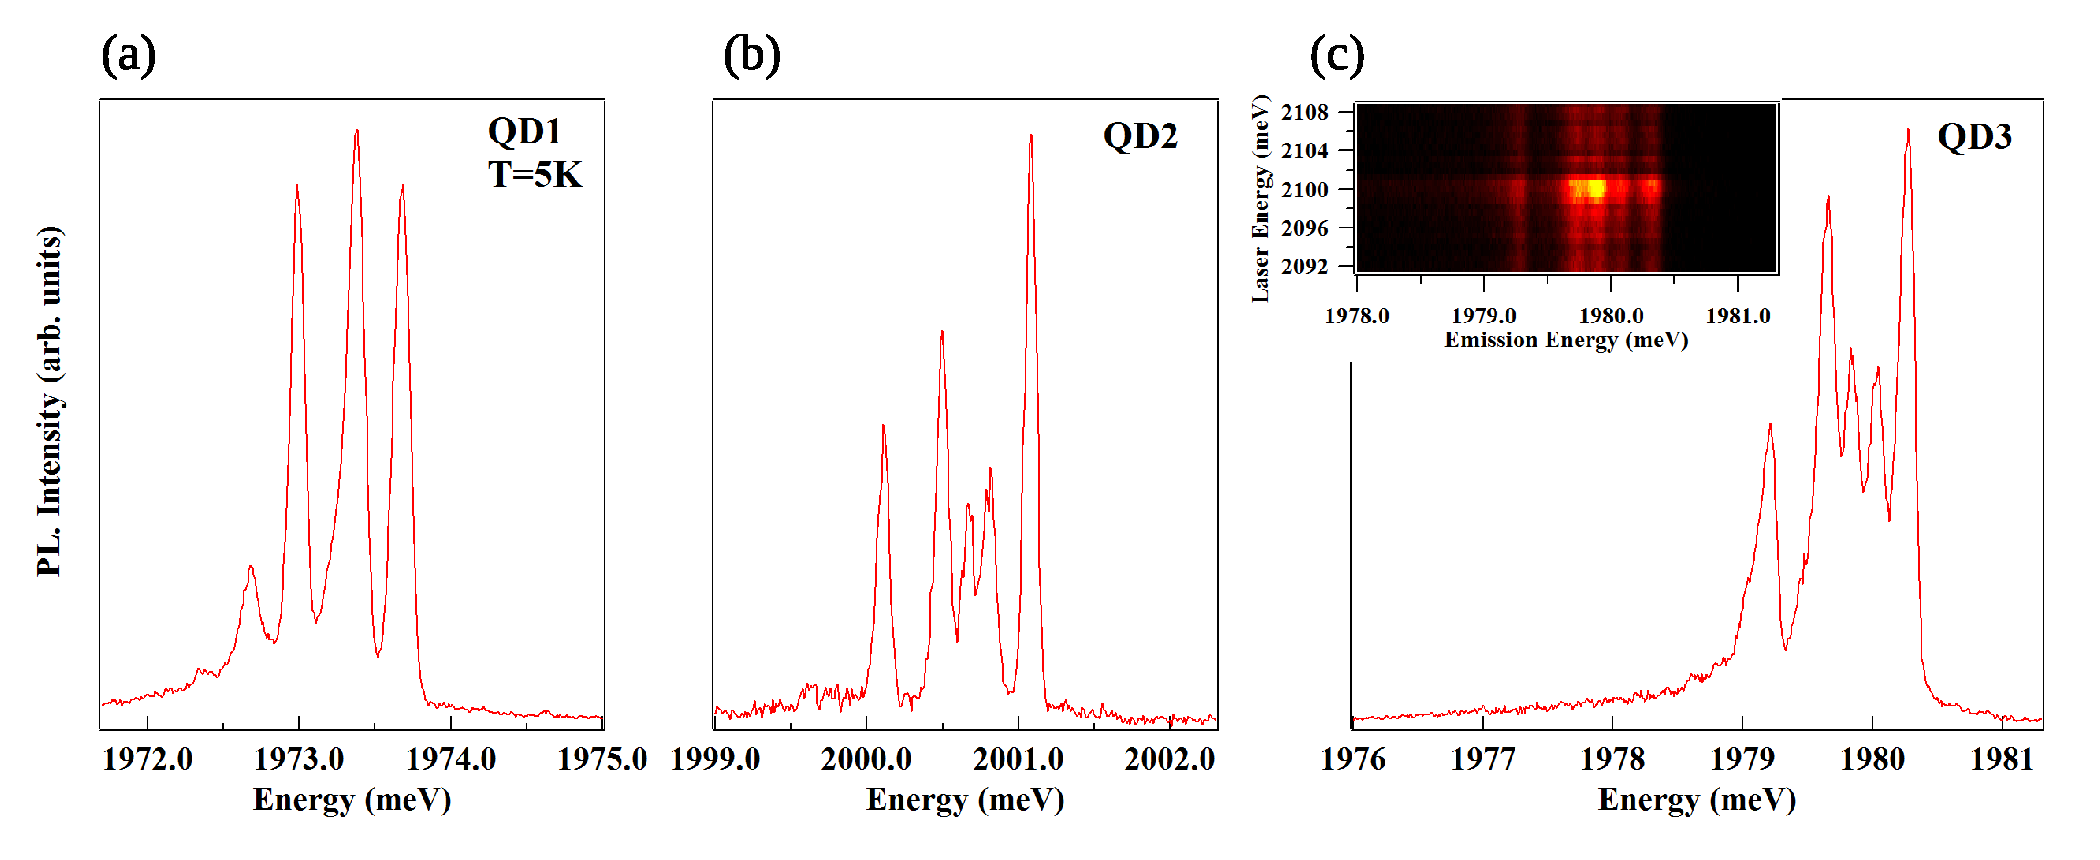
\includegraphics[width=15cm]{Pictures/Spectras.eps}
	\end{center}
	\caption{PL of X-Cr complex at low temperature (T=5K) for (a) QD1 (found in dot334), (b) QD2 (dot338) and (c) QD3 (dot334). Inset in (c) presents the PLE map of this QD, showing a sharp quasi-resonant state for an excitation at 2100 meV.}
	\label{SpectraX}
	\end{figure}

	Low temperature (T=5K) PL of the neutral exciton (X-Cr) of several QDs doped with a single Cr are reported in Fig.~\ref{SpectraX}. Three main emission lines are observed, with a fourth, weaker peak on the low energy side. In some QDs, such as QD2 and QD3, the central peak is split. Scanning with an energy tunable laser, we saw that all the peaks share a common excited state, as highlighted in the inset of Fig.~\ref{SpectraX}(c). This is an indication that they originate from the same dot. Variations in the relative intensities of the peaks are observed from dots to dots.

	\begin{figure}[h!]
	\begin{center}
		\includegraphics[width=10cm]{Pictures/EnLvlantiferro.png}
	\end{center}
	\caption{Illustration of the energy levels of the ground state (Cr), the bright exciton states ($|\pm1\rangle$) coupled to the spin of a Cr (X-Cr) and dominant PL transitions ($\sigma$+, $\sigma$-). The states $S_z = \pm2$ cannot be populated through thermalization, and thus their recombination channel are not shown on this schema.}
	\label{CrEnergyStruct}
	\end{figure}

	As we have seen in Sec.~I.3.2%~\ref{CrSemiCon}
, in a II-VI semiconductor, the orbital momentum of the Cr connects the spin of the atom to its local strain environment through the modification of the crystal field and the spin-orbit coupling. For biaxial strain in the (001) plane, the ground state of a Cr spin is split by a strain induced magnetic anisotropy term ${\cal H}_{Cr,\varepsilon_\parallel}=D_0S^2_z$. It was deduced from electron paramagnetic resonance of bulk Cr-doped CdTe that $D_0$ is positive for compressive biaxial strain~\cite{EPRCr}. In a self-assembled CdTe/ZnTe QDs with large in-plane strain, the Cr levels $S_z=0$, $\pm1$ and $\pm2$ split parabolically (Fig.~\ref{CrEnergyStruct}). A value of $D_0$ in the meV range can be expected for a CdTe layer strained on a ZnTe substrate, as shown in Sec.~\ref{CrSemiCon}.
	
	\begin{figure}[h!]
	\begin{center}
		\includegraphics[width=14.5cm]{Pictures/LinPol.png}
	\end{center}
	\caption{(a) Low temperature (T = 5 K) PL of QD2 recorded in linear polarization along two orthogonal directions. (b) Linear polarization PL intensity map of QD2. The 0$^{\circ}$ polarization angle corresponds to an emission polarized along the QD cleavage axis, either $[110]$ or $[1\bar{1}0]$. (c) Illustration of the energy levels of the ground state (Cr), the bright exciton states ($|\pm1\rangle$) coupled to the spin of a Cr (X-Cr), showing the splitting of the central peak via the bright exciton coupling, and dominant PL transitions: $\sigma$+ in blue, $\sigma-$ in red and $\pi$ in green and black.}
	\label{CrLinPolar}
	\end{figure}
	
	When an electron-hole pair is injected in a Cr-doped QD, the bright excitons are split by the exchange interaction between the spins of Cr and carriers. In flat self-assembled QDs, the heavy-holes and light-holes are separated in energy by the biaxial strain and the confinement. In a first approximation, the ground state in such QD is a pure heavy-hole ($J_z$=$\pm$3/2) exciton and the exchange interaction with the Cr spin S is described by the spin Hamiltonian 
	\begin{align}
		{\cal H}_{c-Cr}=I_{eCr}\mathbf{S}\cdot\bm{\upsigma}+I_{hCr}S_zJ_z
	\end{align}		
with $\bm{\upsigma}$ the electron spin and $J_z$ the hole spin operator. $I_{eCr}$ and $I_{hCr}$ are, respectively, the exchange integrals of the electron and the hole spins with the Cr spin. These exchange energies depend on the exchange constant of the Cr $3d$ electrons with the CdTe carriers and on the overlap of the Cr atom with the confined carriers. Even though the exchange interaction of the Cr spin with both electron and hole is ferromagnetic in bulk II-VI semiconductor studied until now~\cite{MacCdCrSD0beta,KacmanD0alphabetaIIVI,MacspdexchCr}, the hole-Cr interaction is supposed to be anti-ferromagnetic here. This does not change the structure of the PL at B = 0T. The only visible effect of the sign of the exchange interaction will be on the PL intensity distribution in the magneto-optics experiments. This choice of sign of the hole-Cr exchange interaction will be further discussed in Sec.~\ref{MagOptCr}. A typical exchange constant 4 to 5 times larger for the holes than for the electrons is also expected in CdTe~\cite{DMSCrExchInt,CdCrSExchInt}.

	\begin{figure}[h!]
	\begin{center}
		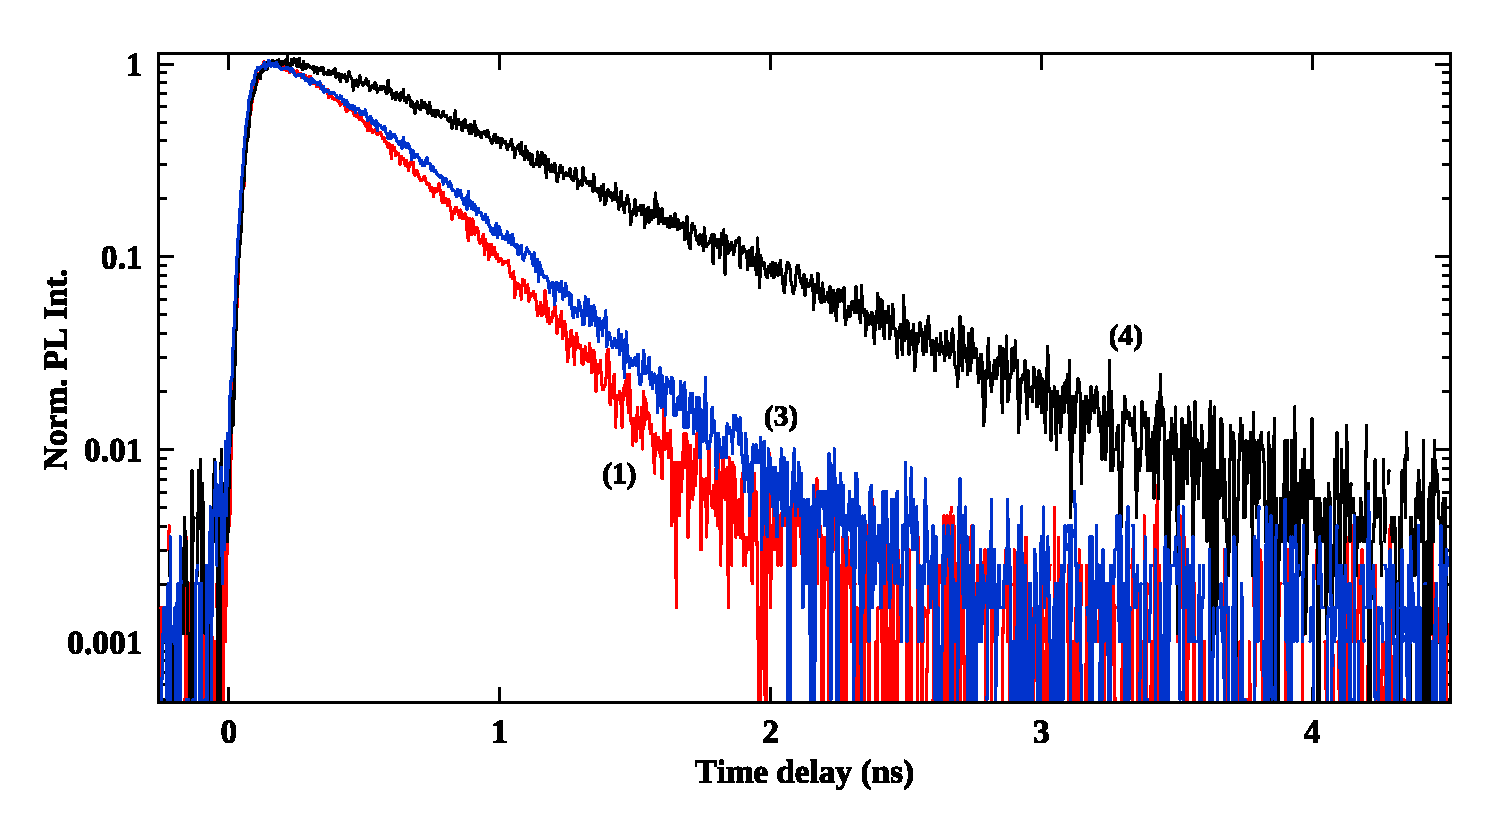
\includegraphics[width=12cm]{Pictures/Decay.eps}
	\end{center}
	\caption{Time resolved PL of QD2 taken on two outside peaks at T = 5 K, attributed to $S_z = \pm1$ (noted (1) and (3) in Fig.~\ref{CrLinPolar}(a)), and the lower energy one (noted (4)).}
	\label{CrDecay}
	\end{figure}
	
	For highly strained CdTe/ZnTe QDs with a weak hole confinement, the strain induced energy splitting of the Cr spin $D_0S^2_z$ is much larger than the exchange energy with the confined carriers ($D_0\gg |I_{hCr}|>|I_{eCr}|$). The exchange interaction with the exciton acts as an effective magnetic field which further splits the Cr spins states $S_z=\pm$1 and $S_z=\pm$2. The resulting X-Cr energy levels are presented in Fig.~\ref{CrEnergyStruct}. The exciton recombination does not affect the Cr atom and its spin is conserved during the optical transitions. Consequently, the large strain induced splitting of the Cr spin is not directly observed in the optical spectra. However, at low temperature, the Cr spin thermalize on the low energy states $S_z$=0 and $S_z$=$\pm$1. This leads to a PL dominated by three contributions: a central line corresponding to $S_z=0$ and the two outer lines associated with $S_z=\pm$1 split by the exchange interaction with the carriers.
	
	Most of the Cr-doped quantum dots exhibit a linear polarization dependence, as presented in Fig.~\ref{CrLinPolar}. The central line ($S_z$=0) is split and linearly polarized along two orthogonal directions. As in non-magnetic QDs, this results from a coupling of the two bright excitons $|\pm1\rangle$ by (i) the long-range e-h exchange interaction in a QD with an in-plane shape anisotropy~\cite{SplitInvTh} and/or (ii) the short range e-h exchange interaction in the presence of valence band mixing. This anisotropic e-h exchange energy mixes the bright exciton associated with the same Cr spin state, inducing an extra splitting between them. The mixing is maximum for the central pair of bright excitons (S$_z$=0) which are initially degenerated. The outer lines are also slightly linearly polarized but the influence of the e-h exchange interaction is attenuated by the initial splitting of the $|\pm1\rangle$ excitons induced by the exchange interaction with the Cr spin $S_z=\pm1$.	

	In order to identify the nature of the lower energy peak ((4) in Fig.~\ref{CrLinPolar}(a)), we performed time resolved PL experiments on the emission peaks (1), (3) and (4). The results, presented in Fig.~\ref{CrDecay}, show that the line (4) presents a decay time about twice longer than the other lines. Such a long decay time is consistent with the radiative recombination of a dark exciton. Under normal circumstances, the recombination of such a state is forbidden. However, in QDs with a symmetry lower than C$_{2v}$ (truncated ellipsoidal lens for example), the bright and dark exciton states can get mixed. It is then possible to observe a dark exciton emitting a photon~\cite{DELum,DERecombTh}. Since it is initially a forbidden transition, the recombination will be less efficient and will thus take more time~\cite{DELongLifetime}. This hypothesis will be confirmed by the magneto-optical study of the dot presented in Fig.~\ref{CrMagOptExp} and \ref{CrMagOptMod}.
	
	\begin{figure}[h!]
	\begin{center}
		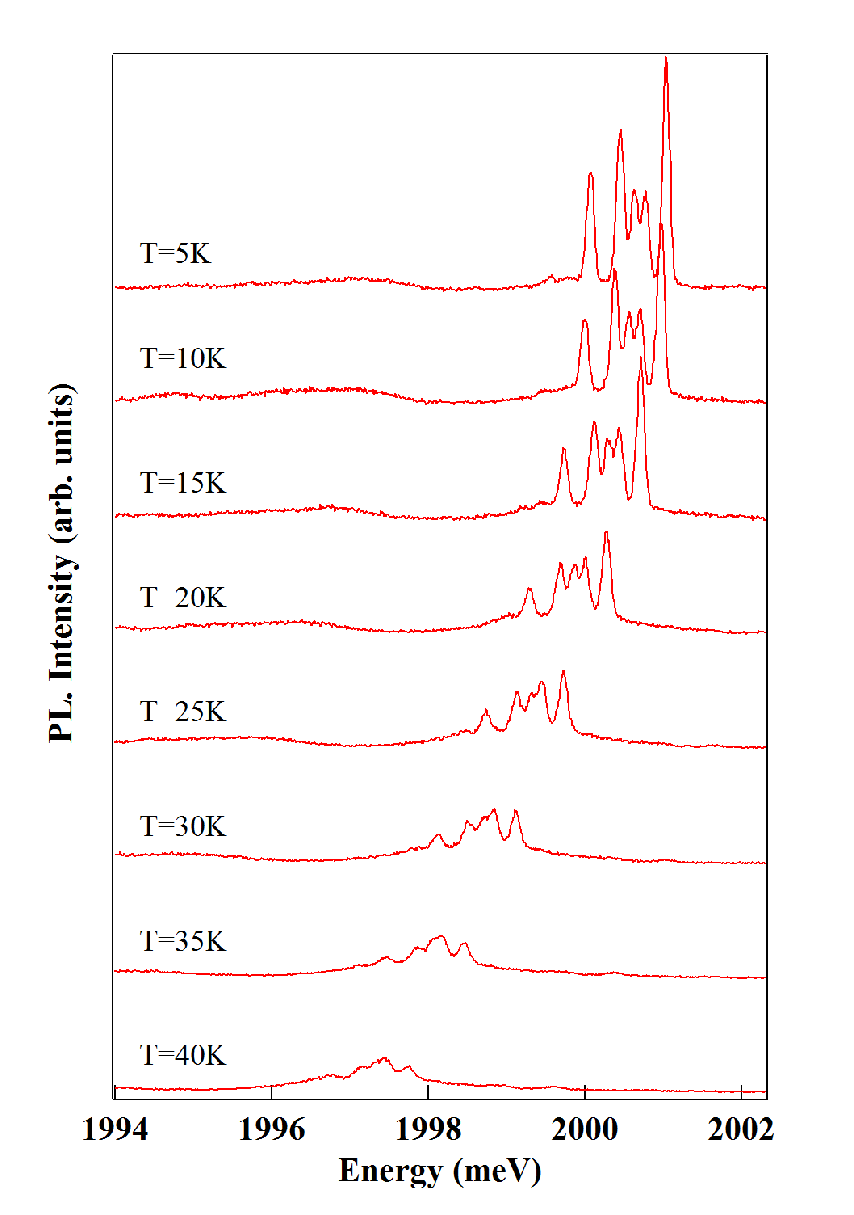
\includegraphics[width=14.9cm]{Pictures/Temp.eps}
	\end{center}
	\caption{Temperature evolution from T=5K to T=40K of (a) the PL of QD2 and (b) the PL of a QD with a good thermalisation on the low energy states (QD4).}
	\label{CrTemp}
	\end{figure}
	
	Since the Cr spin states $S_z = \pm2$ do not appear on the PL because they cannot be thermally populated at T = 5K, one could expect to see their emission at higher temperature. Fig.~\ref{CrTemp} presents the emission of two dots as a function of the temperature. With the increase of the temperature, we observe a significant line broadening induced by the interaction with acoustic phonons~\cite{BesombesAccPhon}. In order to keep a significant PL intensity and resolved PL lines, we limited our investigation to temperature below 40K. Even at this temperature, the PL peaks corresponding to $S_z = \pm2$ does not appear. However, the structure of the emission change slightly with the temperature. The intensity of the outside peaks, associated with the states $S_z = \pm1$, decreases faster than the intensity of the PL peak associated with $S_z = 0$ when the temperature increases. This is an unexpected picture, since a higher temperature should allow the higher energy states $S_z = \pm1$ to be more populated by emptying the ground state when increasing. To explain this behaviour on the low energy peak, we propose that the state $S_z = 0$ is partly populated by a h-Cr spins flip-flop from the states $S_z = \pm1$ coupled to the dark states. This process is explained with more details in Sec.~V.3.1%~\ref{hCrff}
. When the temperature rises, the probability for the dark states to recombine non-radiatively increases, and thus the decrease of the population and PL intensity of the peaks associated with the state $S_z = 0$ would be slower than the intensity of the one associated with $S_z = \pm1$.
	%\newpage

%	\begin{sidewaysfigure}
%	\begin{center}
%		\includegraphics[width=20cm]{Pictures/FullPLE}
%	\end{center}
%	\caption{(a) Map of QD2 PL under a scan in laser energy close to the dot emission in $\sigma -$ detection. Several interesting points are highlighted on zoom on each side of this whole map. (b) Map of the first few meV of the scan, showing the phonon replica. The emission integrated intensity as a function of the laser energy is plotted in (c) (black curve) along with the PL spectra of QD2 (red curve). (d) - (f) present a zoom in a larger band at higher excitation energy in $\pi$,  $\sigma +$ and $\sigma -$ respectively. (g) Zoom on a particular excited state presented a splitting inversion, presented here in $\pi$ detection.}
%	\label{CrPLE}
%	\end{sidewaysfigure}

		\subsection{Excited states of a Cr-doped QD}	
	
	The excited states in QD2 were investigated by PLE, starting close to the energy of the dot's emission. The data reported in Fig.~\ref{FullPLE}(a) present several excited states at different excitation energy.
	
	\begin{figure}[h!]
	\begin{center}
		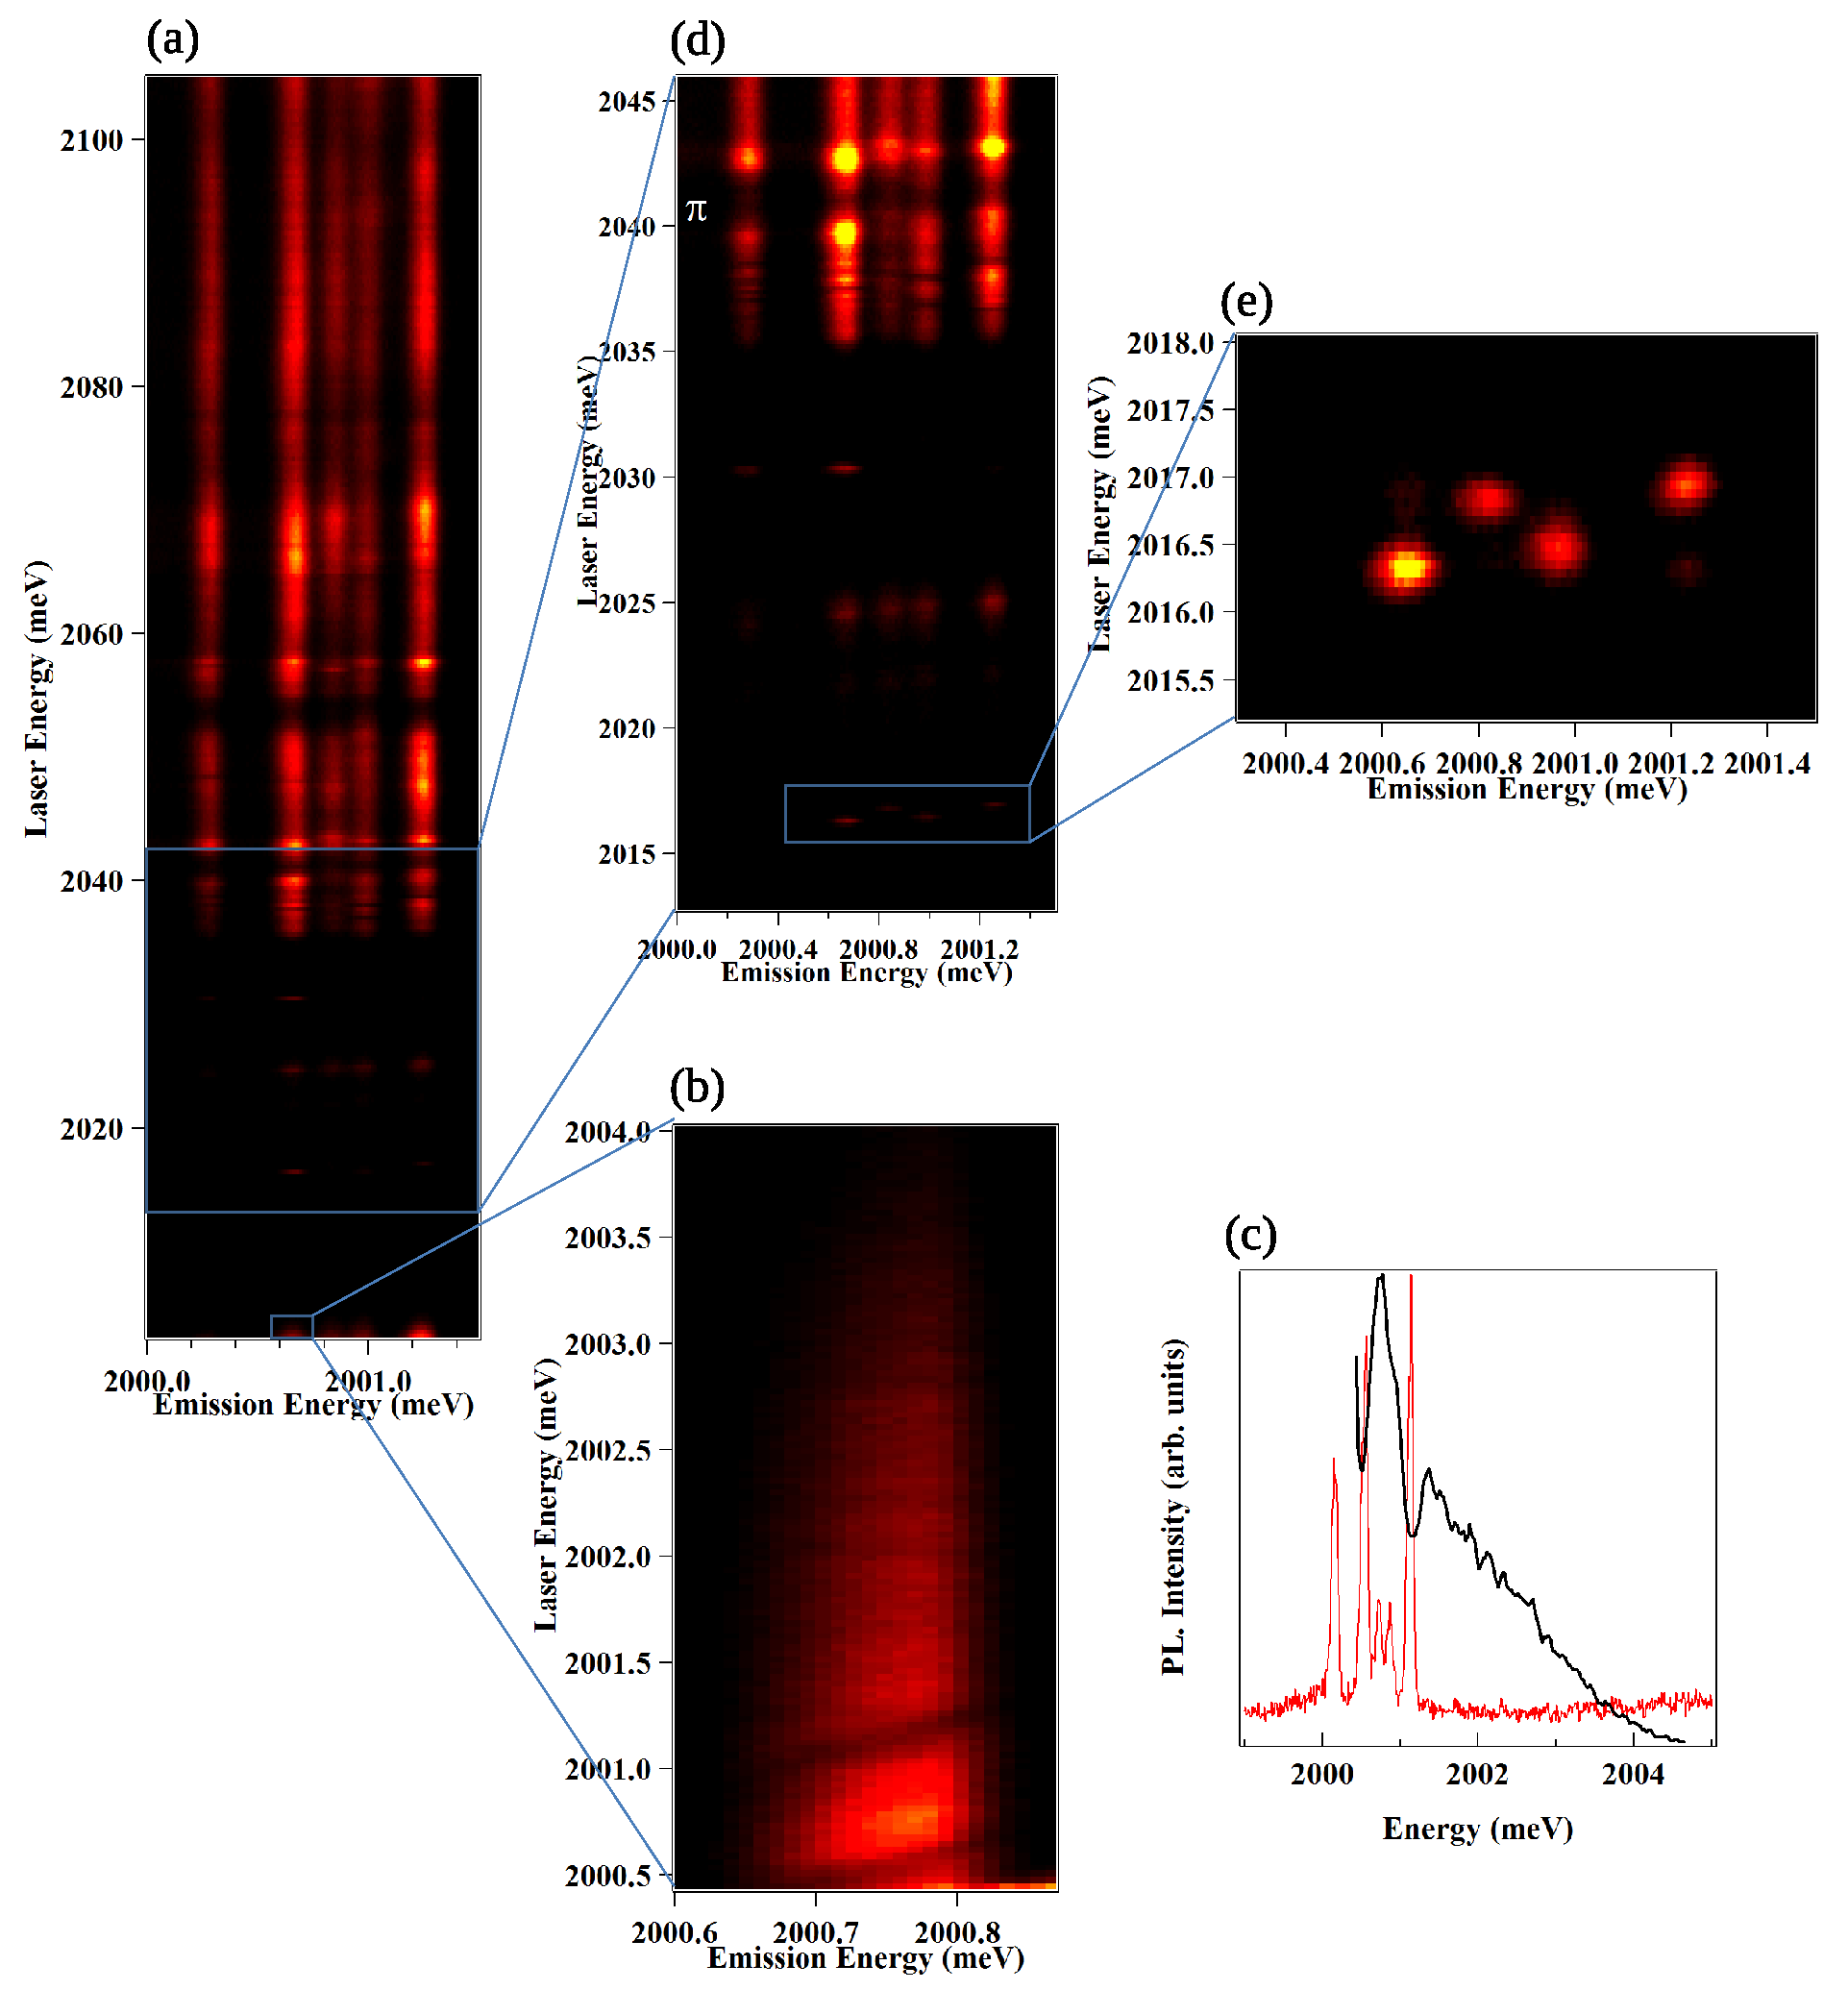
\includegraphics[width=13.8cm]{Pictures/FullPLEv2.eps}
	\end{center}
	\caption{(a) QD2 X-Cr PLE map at T = 5 K in $\pi_{cross}$ polarization. Several excited states are highlighted. (b) Photoluminescence of QD2 X-Cr complex for an excitation at 2120 meV). (c) PLE scan detected on the lower energy peak, taken close to the QD emission energy, showing the phonon replica taken in $\pi$ cross excitation/detection. The emission integrated intensity as a function of the laser energy is plotted in (d) (black curve) along with the PL spectra of QD2 taken in $\sigma_{co}$ polarization. (e) PLE map between 2046 meV and 2013 meV presenting several excited states, detecting in $\pi_{cross}$ polarization. (f) Zoom on a particular excited state presenting a splitting inversion, taken in $\pi_{cross}$ detection.}
	\label{FullPLE}
	\end{figure}
	
	Starting at low excitation energy, the first noticeable thing on this scan is the PL observed over a large excitation energy range, for an excitation between the dot emission energy (between 2000 and 2001 meV) and 2004 meV. A zoom is presented in Fig.~\ref{FullPLE} (c) for a detection on the dark exciton line. This absorption band corresponds to an excitation of the QD via the acoustic phonon side band. 
%	When on this band, the laser heat the sample, creating phonon in the absorption band on the dot.	The phonons will be able to excite the dot, generating an exciton inside and thus triggering the photoluminescence [A VERIFIER].
One can notice two sharp intensity decreases in this emission. Comparing the integrated intensity of the PL of the dark state during the laser scan with the QD spectra (Fig.~\ref{FullPLE}(d)), it appears that those two intensity drops happen when the laser is in resonance with a QD emission line. The resonantly excited state saturate the absorption, reducing strongly the absorption in the dark exciton phonon side band.

%	\begin{figure}[h!]
%	\begin{center}
%		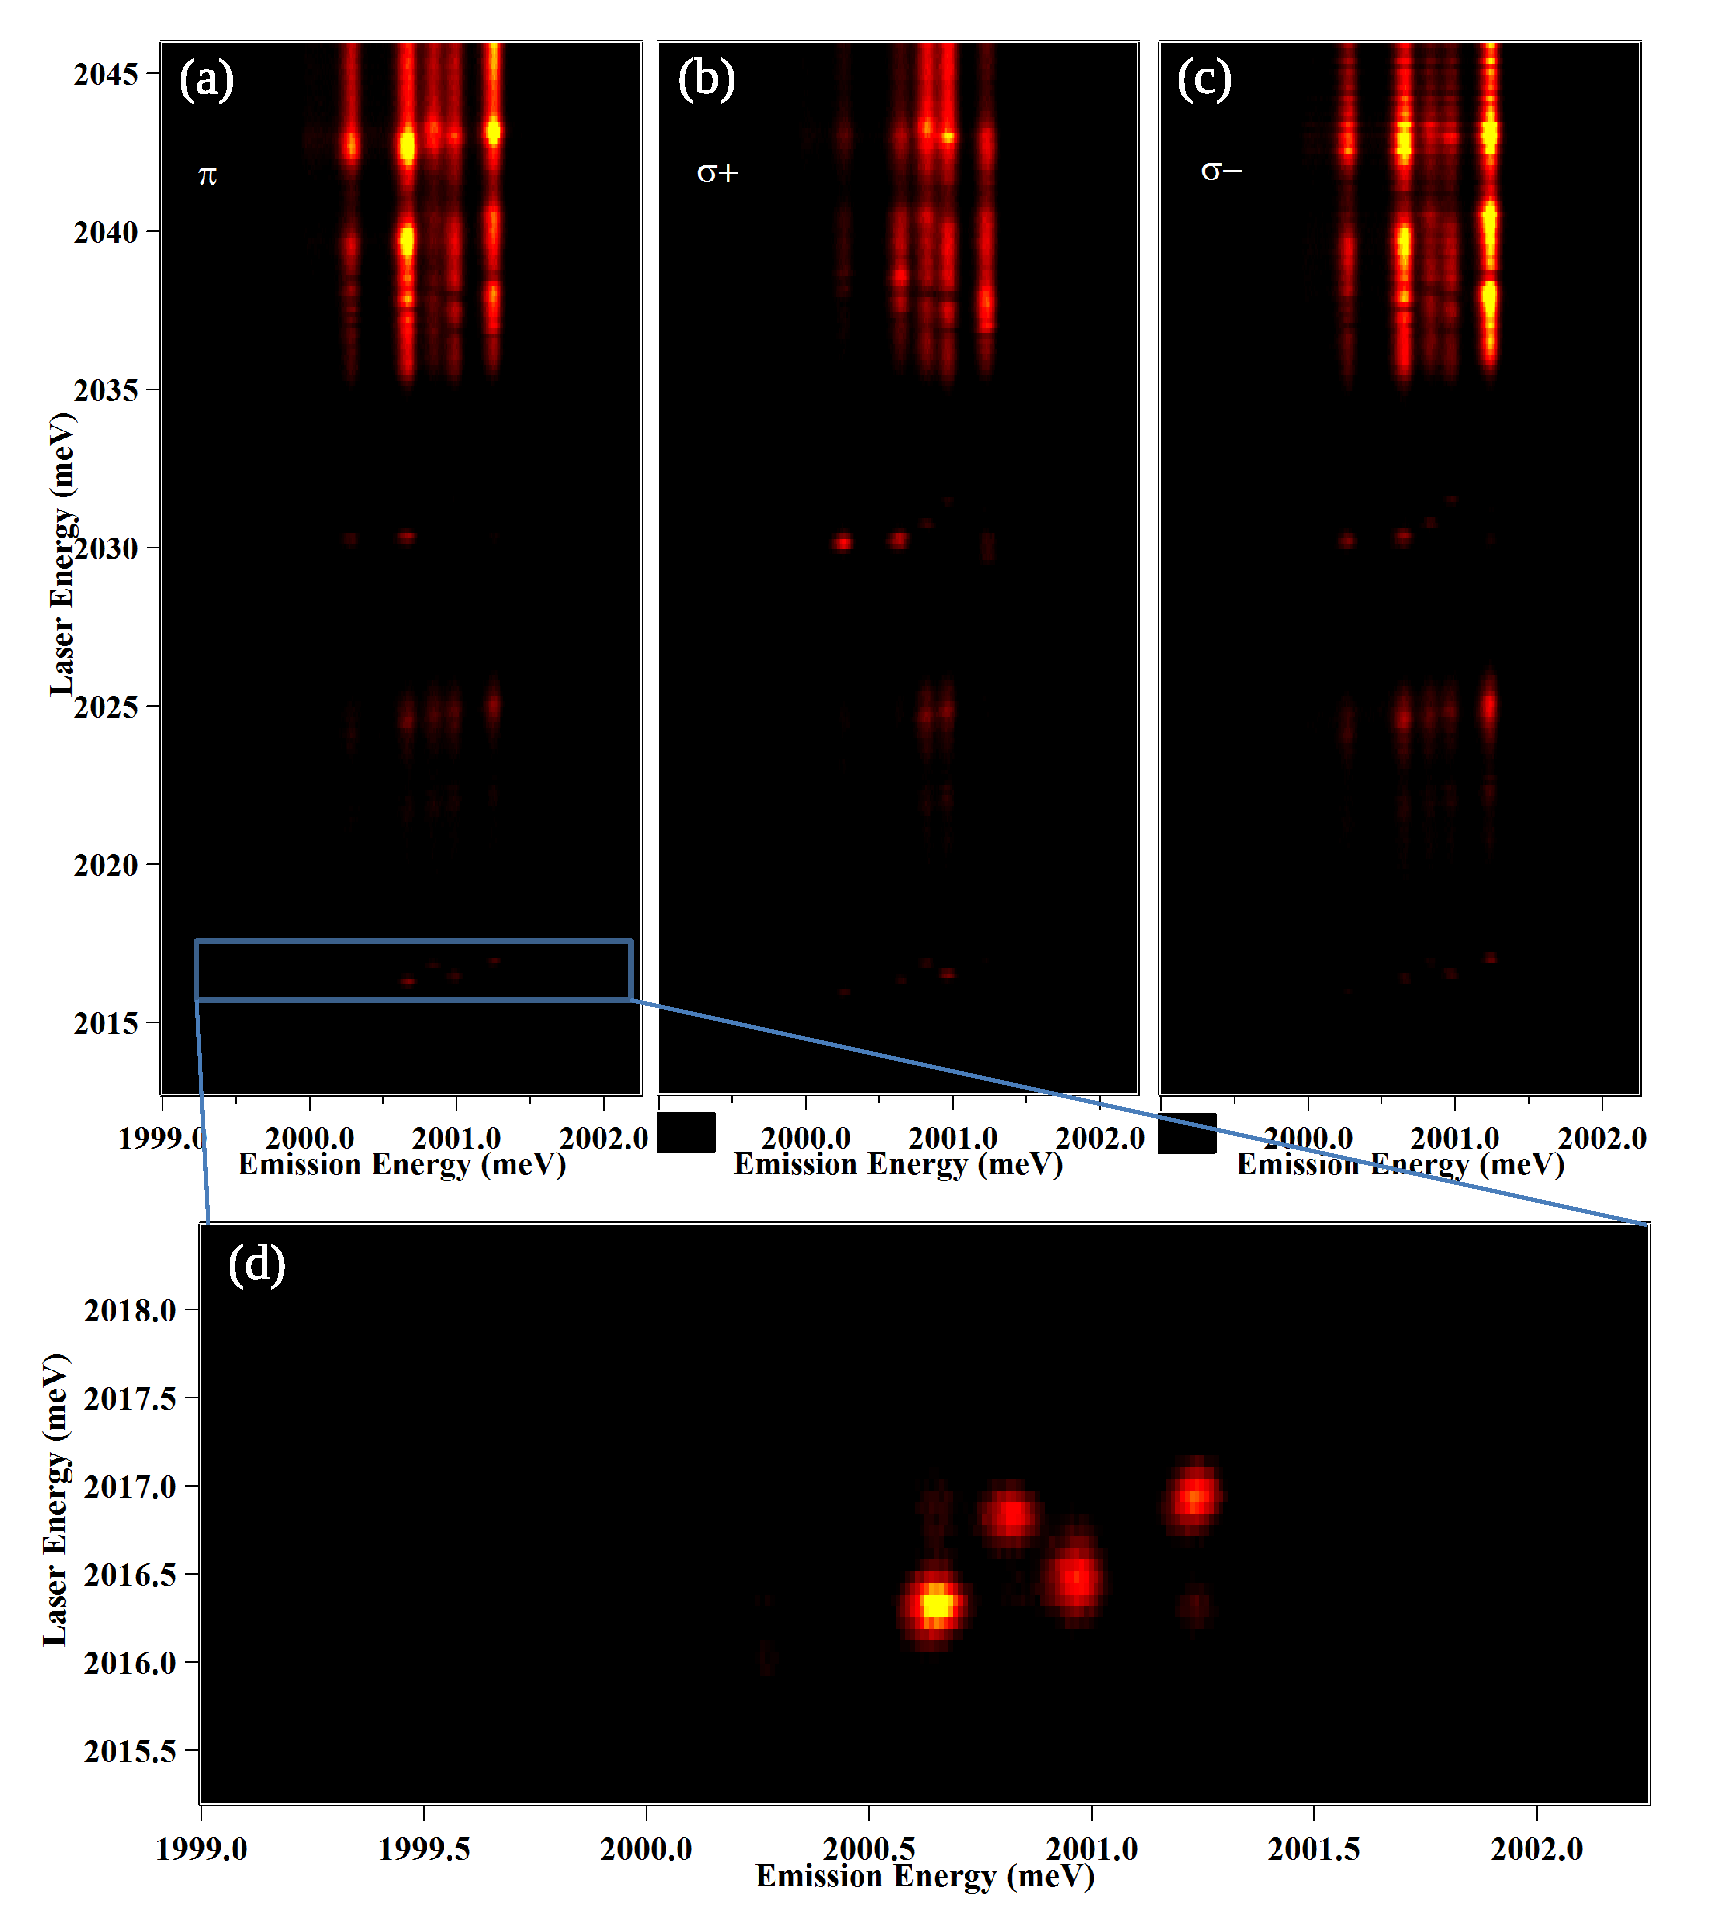
\includegraphics[width=12cm]{Pictures/PLE2030.eps}
%	\end{center}
%	\caption{(a) - (c) PLE map between 2046 meV and 2013 meV presenting several excited, detecting in $\pi$ (a),  $\sigma_{co}$ (b) and $\sigma_{cross}$ (c). (d) Zoom in a particular excited state presented a splitting inversion, taken in $\pi$ detection.}
%	\label{PLE2030}
%	\end{figure}
	
	Another excited state appears around 2018.5 meV, presented in Fig.~\ref{FullPLE} (f). The first feature of this peak is that, each of the peak here presents a slightly different resonant energy. Moreover, one can note that the order of appearance during the energy scan of the two central peaks is reversed compared to the external ones. For the outside peaks, the low energy one appears before the high energy one. This order is inverted for the central peaks. Such splitting inversion, was first observed on QDs in GaAs quantum well~\cite{FineStructSplitGaAsdots}. It has been discussed by Takagahara~\cite{SplitInvTh} and is due to the electron-hole exchange interaction in anisotropic potential.
	
	\begin{figure}[h!]
	\begin{center}
		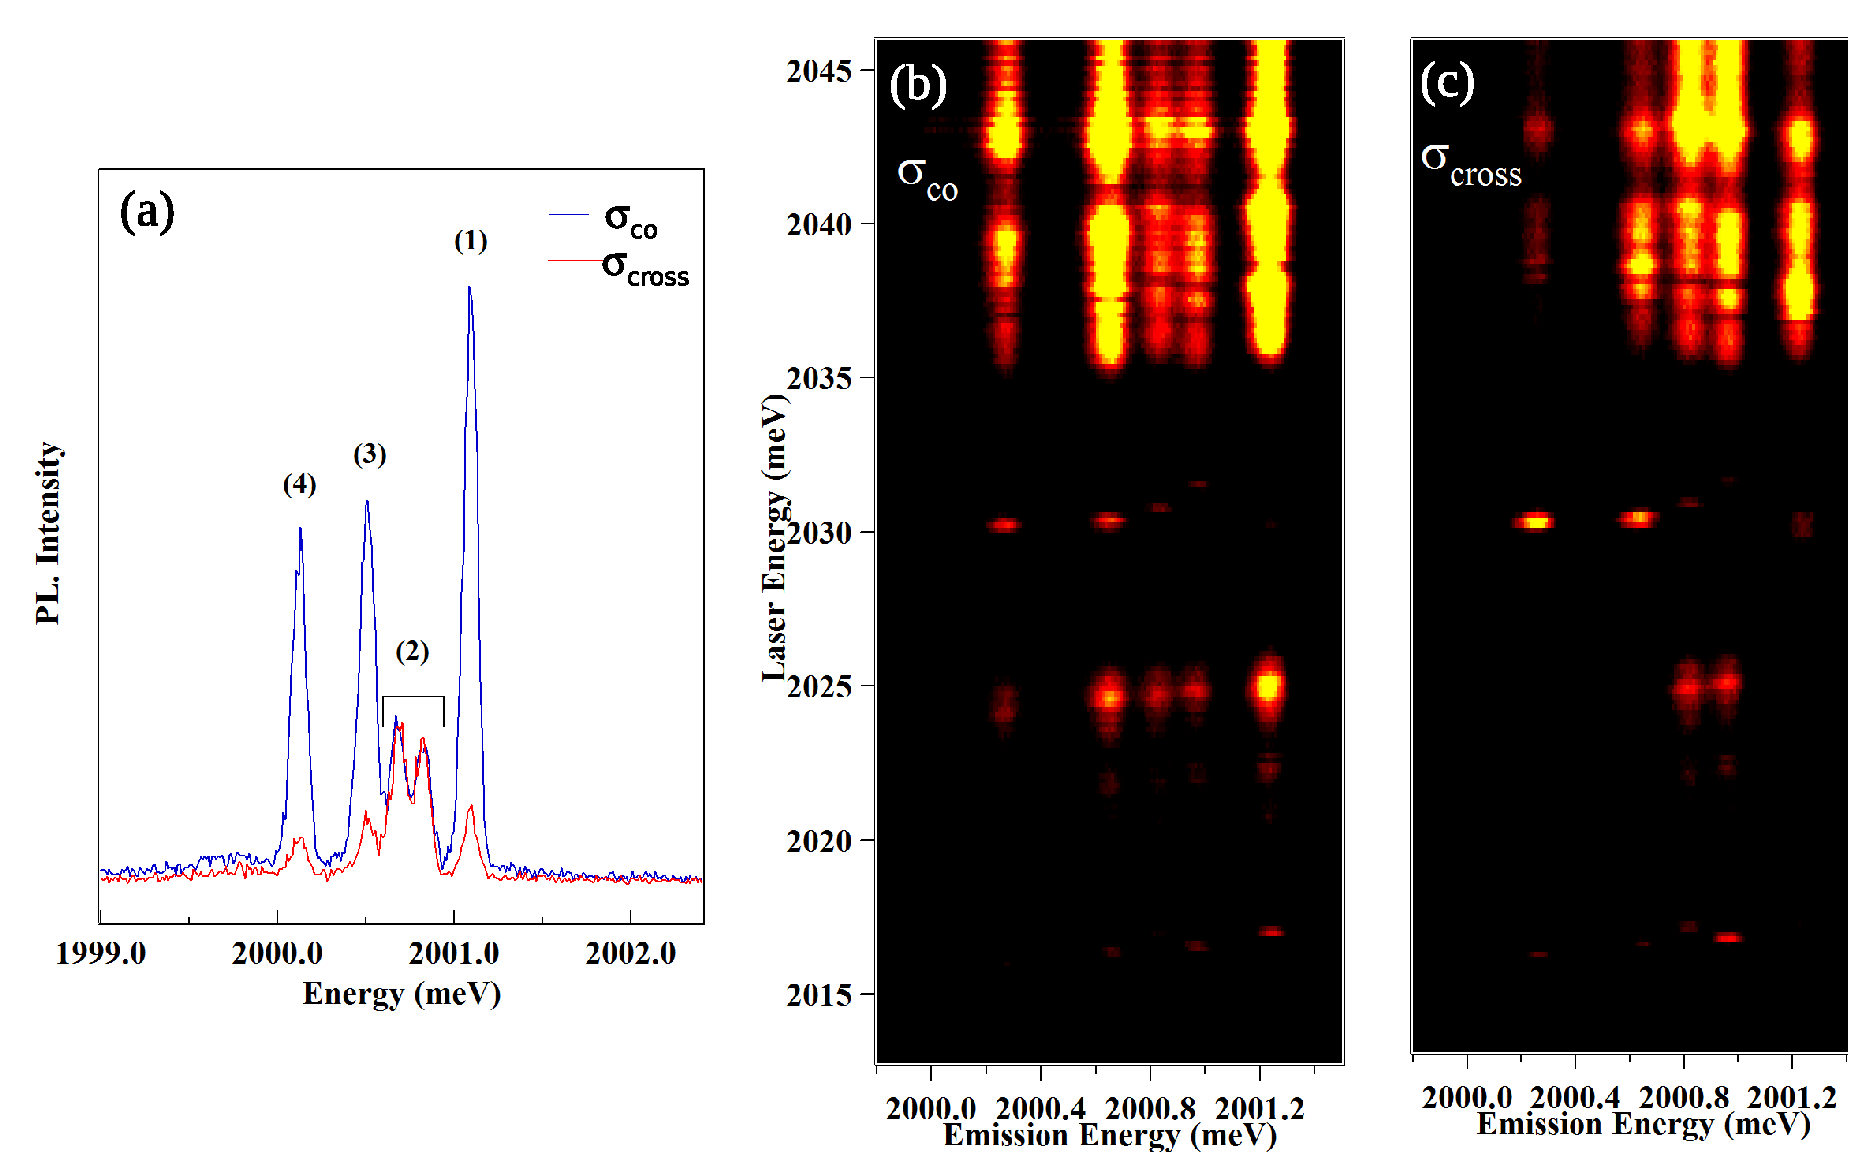
\includegraphics[width=14.9cm]{Pictures/PLEDotPres.eps}
	\end{center}
	\caption{(a) Low temperature (T = 5 K) PL spectra of the exciton in QD2 (X-Cr) for co-circularly (blue) and cross-circularly (red) polarized excitation/detection taken for an excitation around 2120 meV. (b) - (c) PLE map at T = 5 K between 2046 meV and 2013 meV presenting several excited states, detected in $\sigma_{co}$ (b) and $\sigma_{cross}$ (c).}
	\label{PLEDotPres}
	\end{figure}
	
	The next excited state can be seen at 2025 meV, more visible on ~\ref{FullPLE} (e). It can be linked to an excitation through optical phonons. Looking at the $\sigma$ polarized emissions for an excitation on these states (Fig.~\ref{PLEDotPres}(b) and (c)), we can see that the low and high energy peaks are strongly $\sigma_{co}$ polarized. It means that the exciton recombines in the same spin as the one injected by the laser. It shows that the spin of the exciton in the QD is conserved during its lifetime. This stabilization of the exciton spin is due to the Cr spin acting as an effective magnetic field. The split central peak is linearly polarized, as discussed in Sec.~\ref{CrPres}. As expected, its emission shows no dependency in circular polarization in Fig.~\ref{PLEDotPres}. 
	
	Finally, another interesting excited state appear at 2030 meV. This state presents a different exchange-induced splitting than the splitting in the excited state around 2100 meV presented in Fig.~\ref{SpectraX}. This is due to a difference in the carriers and Cr atom wavefunction overlap.

		\subsection{Magneto-optics of QDs doped with a single Cr atom\label{MagOptCr}}
		
	The structure of the energy levels of Cr-doped QDs presented in Fig.~\ref{CrEnergyStruct} is confirmed by the evolution of the PL spectra in magnetic field, up to 11 T, along the growth axis, the so called Faraday configuration~\cite{BesombesPumpMnSFD}, presented in Fig.~\ref{CrMagOptExp}. When applying such a magnetic field, the bright exciton $X_z = \pm1$ splits, leading to a $\sigma-$ branch shifting at low energy and a $\sigma+$ one shifting at high energy. This splitting can compensate the one induced by the exchange interaction with the Cr~\cite{LegerQDGeomEffect}. For QD1, this results in an anti-crossing of $|+1\rangle$ and $|-1\rangle$ excitons due to the e-h exchange interaction around B$_z$=6 T observed both in $\sigma+$ and $\sigma-$ polarizations (anti-crossing (2) and (3) in Fig.~\ref{CrMagOptExp}(a)).
		
	\begin{figure}[h!]
	\begin{center}
		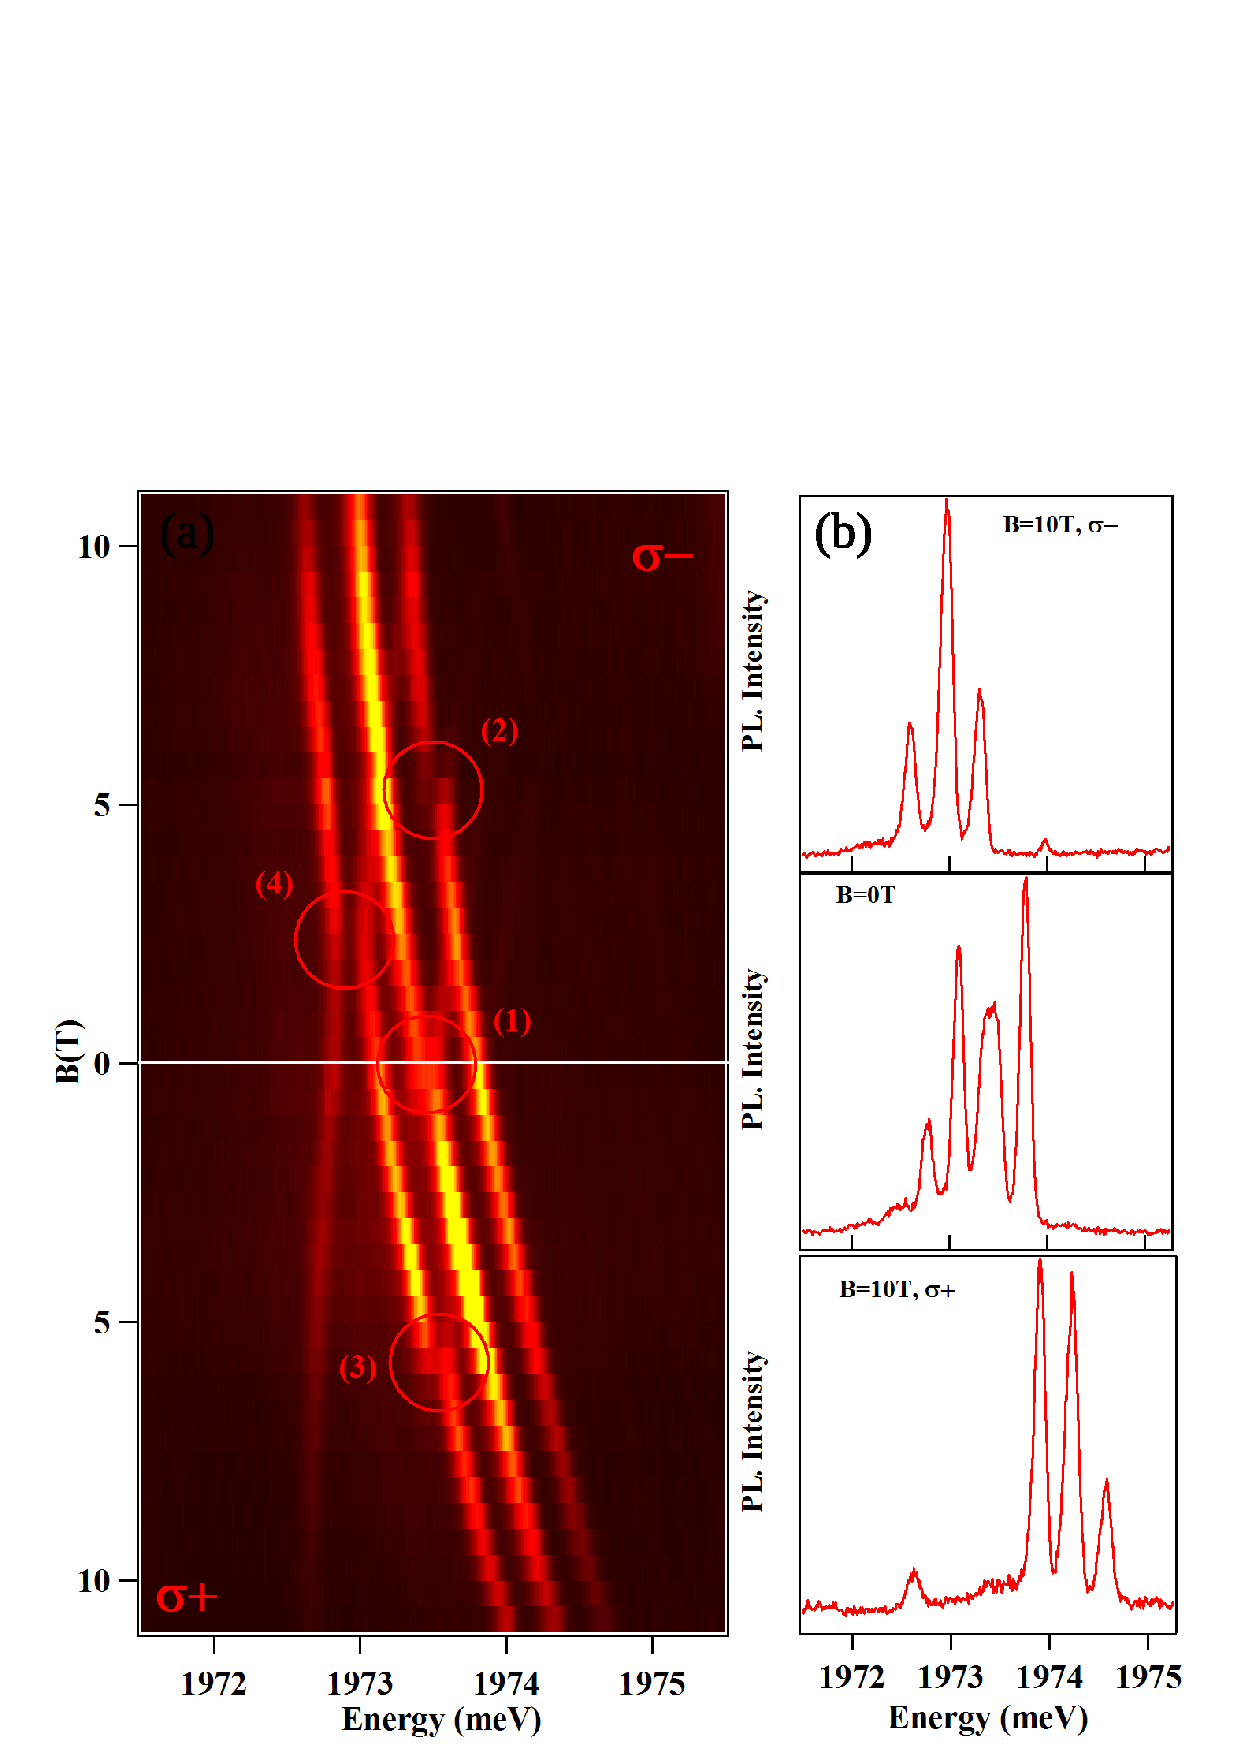
\includegraphics[width=10cm]{Pictures/MagOptv2.png}
	\end{center}
	\caption{(a) Evolution of the circularly polarized X-Cr PL of QD1 under magnetic field applied along the growth axis ($B_z$) at T = 5 K. ASee text for the identification of the anti-crossing (1), (2), (3) and (4). (b) Corresponding PL spectra taken at 0 and $10$T for both circular polarization.}
	\label{CrMagOptExp}
	\end{figure}
		
		The low energy emission presented as a dark exciton in Fig.~\ref{CrDecay} shows an anti-crossing with the bright excitons under $B_z$ in $\sigma-$ polarization (anti-crossing (4) in Fig.~\ref{CrMagOptExp}). This anti-crossing arises from a mixing of the bright and dark excitons interacting with the same Cr spin state. When detecting in $\sigma-$ polarization, it corresponds to the mixing of the exciton states $|-1\rangle$ and $|+2\rangle$ coupled to the Cr spin $S_z=+1$. This dark/bright excitons coupling $\delta_{12}$ is induced by the e-h exchange interaction in a confining potential with a symmetry lower than C$_{2v}$~\cite{DERecombTh}. In such symmetry, the dark exciton acquire an in-plane dipole moment which leads to possible optical recombination at zero magnetic field~\cite{DELum}. The oscillator strength of this "dark exciton" increases as the initial splitting between $|-1\rangle$ and $|+2\rangle$ excitons is reduced by the magnetic field.
		
	\begin{figure}[h!]
	\begin{center}
		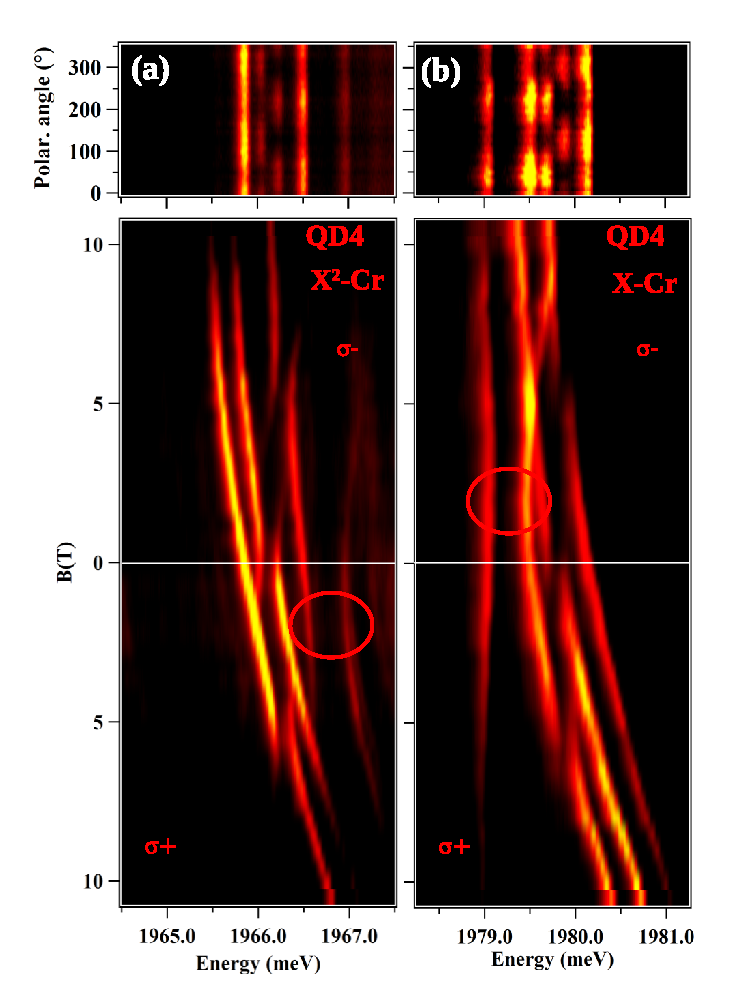
\includegraphics[width=10cm]{Pictures/MagOptLowSym.eps}
	\end{center}
	\caption{Linear polarization intensity map (a) X$^2$-Cr and (c) X-Cr in QD3. (b) - (d) Respective intensity map of the longitudinal magnetic field dependence of the emission (bottom panel) of }
	\label{CrMagOptLowSym}
	\end{figure}
		
		To illustrate the influence of the QD symmetry on the magneto-optical properties of X-Cr, we show in Fig.~\ref{CrMagOptLowSym}(b) the emission of a QD with a different strain or shape anisotropy (QD3). For QD1, the splitting of the central peak is not clear in the PL at 0T (Fig.~\ref{SpectraX}(a)), while two linearly polarized peaks appear in QD3 spectra (Fig.~\ref{SpectraX}(c)).
%		This difference in emission arises from a difference in the in-plane strain anisotropy of each QD~\cite{SplitInvTh}.
		
		Investigating both the biexciton and the exciton in the same Cr-doped QD, we can also analyze the impact of the carrier-Cr interaction on the fine structure of the Cr spin. The magnetic field dependence of X$^2$-Cr emission in QD3 is presented along with the X-Cr emission as a contour plot in Fig.~\ref{CrMagOptLowSym} (a) and (b) respectively. The PLs under magnetic field of X-Cr and X$^2$-Cr present a mirror symmetry. In particular, the dark/bright exciton mixing observed around $B_z=2.5$ T on the low energy side of the PL in $\sigma-$ polarization for X-Cr is observed on the high energy side in $\sigma+$ polarization for X$^2$-Cr (circles in Fig.~\ref{CrMagOptLowSym}(a) and (b)).
		
	\begin{figure}[h!]
	\begin{center}
		\includegraphics[width=13cm]{Pictures/Antiferro-Cr.png}
	\end{center}
	\caption{(a) Evolution in magnetic field of QD4 X-Cr circularly polarized PL. (b) QD3 X-Cr PL at $B_z = 0$ T and $B_z = 7$ T in both polarization. A schema presenting the spin configuration for the most intense outer peak under magnetic field is joined on the side.}
	\label{CrAntiferro}
	\end{figure}
		
		If one considers the ground state of X$^2$ as a spin-singlet (total spin 0), it cannot be split by the magnetic field or the spin interaction part of the carriers-Cr hamiltonian. The creation of two excitons in the QD cancels the exchange interaction with the Cr atom. Thus, the PL of  X$^2$-Cr is controlled by the final state of the optical transitions, i.e. the eigenstates of X-Cr, resulting in the observed mirror symmetry in the PL spectra.
		
	\begin{figure}[h!]
	\begin{center}
		\includegraphics[width=10cm]{Pictures/Antiferro-Mn.eps}
	\end{center}
	\caption{(a) Evolution in magnetic field of the PL of a single Manganese atom coupled to an exciton in a II-VI QD. (b) PL spectra of the X-Mn system taken at $B_z = 0$ T and $B_z = 11$ T in both circular polarization. These experimental results are taken from Yoan L\'eger PhD thesis~\cite{YoanTh}.}
	\label{MnAntiferro}
	\end{figure}
		
	The sign of the interaction between the Cr and the hole spin can be found by studying the evolution under magnetic field of the relative intensity of each of the QD peaks. As shown in Fig.~\ref{CrEnergyStruct}, for a given polarization, each peak can be linked to a Cr spin state. As discussed earlier, applying a magnetic field lifts the degeneracy between the exciton states and allows to efficiently select the polarization of the emission.
%	For QD1, as shown in Fig.~\ref{CrMagOptExp}, it is difficult to appreciate the variation of the relative intensity of the outside peaks. It hints for a high spin effective temperature, mediated by out of equilibrium phonons, allowing for high energy states to be populated.
	
	QD4, shown in Fig.~\ref{CrAntiferro}, presents a high contrast in the evolution of the intensity under magnetic field and was used to find the sign of the h-Cr exchange interaction. The central peak intensity stays the stronger of the three peaks, whatever the direction of the magnetic field. This is expected, since the $S_z = 0$ state is not affected by the Zeeman effect in this field range. It remains the lower spin state for the Cr atom, and therefore concentrate most of the population. In the $\sigma-$ branch, the high energy peak get brighter while the low energy one disappears for $B_z \geq 8$T. The situation is opposite in the $\sigma+$ branch, where the intensity concentrate on the lower energy peak associated with the bright exciton state.
	
	We will focus in this analysis on the Cr spin states $S_z = \pm1$, associated with the two outside peaks. Under magnetic field, $S_z = -1$ shifts at lower energy, while $S_z = +1$ shifts at higher energy, due to the Zeeman effect with $g_{Cr} \approx 2$. Therefore, at high enough magnetic field, the recombination occurs mainly toward $S_z = -1$. In $\sigma-$ polarization, the spin state $|S_z = -1, X_z = -1\rangle$ is detected. The PL intensity concentrate on the high energy peak, meaning that this state is at high energy. The same analysis can be done for an excitation in $\sigma+$ polarization, detecting the spin state $|S_z = -1, X_z = +1\rangle$: the lower energy line is the most intense, meaning that this state is at low energy. This shows that, in Cr-doped QDs, the evolution of the peaks relative intensities under magnetic field is consistent with an anti-ferromagnetic h-Cr exchange interaction.

	This situation is similar to the one observed in II-VI QDs doped by a single Mn atom, presented in Fig.~\ref{MnAntiferro}. Mn is known to have an anti-ferromagnetic interaction with the hole in CdTe~\cite{GajMnD0alphabeta}. It was shown in \cite{YoanTh} that, under magnetic field, the intensity was mainly on the high energy side when detecting in $\sigma-$ polarization, and on the low energy side in $\sigma+$ polarization.
	%The $S_z = -\frac{5}{2}$ state of the Mn atom was stabilized under magnetic field. From the evolution of the peaks relative intensity and the polarization of the different Mn states, it was then possible to deduce that the interaction between Mn and hole was anti-ferromagnetic.
%	
%	The evolution of the peaks relative intensity for the Cr looks like the one for the Mn. Under magnetic field, the $S_z = -1$ is stabilized, becoming the lower energy state of the doublet $S_z = \pm1$. For a high enough magnetic field, we can only consider the recombination toward $S_z = -1$. The high energy peak corresponds then to the $|S_z = -1, X_z = -1\rangle \rightarrow |S_z = -1\rangle$ on, emitting a $\sigma-$ polarized photon. The low energy one is associate with the $|S_z = -1, X_z = +1\rangle \rightarrow |S_z = -1\rangle$ transition, emitting a $\sigma+$ polarized photon. This is coherent with an anti-ferromagnetic coupling between the Cr and hole, contradicting the assumption made in Sec.~\ref{CrCdTe} and confirming the energy structure presented in Fig.~\ref{CrEnergyStruct}.

	The same evolution was found in our other QDs, even if the evolution of the intensity distribution is less clear. All of this shows that hole-Cr exchange interaction is anti-ferromagnetic in self-assembled CdTe QDs. As was seen in Sec.~I.2.2%~\ref{CrCdTe}
, the sign of this interaction strongly depends on the position of the Cr 3$d$ level relative to the valence band top. This position can be affected by the strains and the confinement. A more detailed modelling is therefore required to explain the hole-Cr anti-ferromagnetic coupling.
		
	\section{Modelization of a Cr-doped QD\label{QDParam}}
	
	The system can be described by a spin effective hamiltonian, that we separate as follows:
	
	\begin{align}
\label{X-Cr} {\cal H}_{X-Cr}={\cal H}_{Cr,\varepsilon}+{\cal H}_{cCr}+{\cal H}_{mag}+{\cal H}_{eh}+{\cal H}_{band}+{\cal H}_{scat}
	\end{align}
where:

${\cal H}_{Cr,\varepsilon}$ describes the fine structure of the Cr atom and its dependency on local strain, as presented in Eq.~I.104%~\ref{Cralone}
. It is mainly drived by $D_0$, the magnetic anisotropy. The in-plane strain anisotropy $E$ has to be small (in the $\mu$eV range) in order for model to reproduce well the data (see Fig.~\ref{CrHighE} for the emission of a dot with a higher E).

\begin{figure}[h!]
	\begin{center}
		\includegraphics[width=14.9cm]{Pictures/SimuAntiferro.png}
	\end{center}
	\caption{(a) Calculated linear polarization PL intensity map of X-Cr at zero field. The 0$^{\circ}$ polarization angle correspond to an emission polarized along the $[100]$ axis. (b) Right: Calculated magnetic field dependency of X-Cr circularly polarized PL. See text for details of the model. Parameters are listed in Tab.~\ref{CrModelParam}. Corresponding anti-crossing are highlighted in the same way as on Fig.~\ref{CrMagOptExp} and \ref{CrAntiferro}. Left: PL spectra calculated for $B_z = 0$ T and $B_z = 11$ T in both circular polarization. The peaks intensity was calculated using only a thermal distribution. (c) Schema of the magnetic field dependency of the energy levels of the low energy Cr spin states $S_z=0$ and $S_z=\pm$1, and corresponding bright ($|+1\rangle$ blue, $|-1\rangle$ red) and dark ($|\pm2\rangle$ green) X-Cr energy levels.}
	\label{CrMagOptMod}
	\end{figure}

${\cal H}_{cCr}$ describes the coupling of the electron and hole with the Cr spin, depending on $I_{eCr}$, the ferromagnetic exchange integral of the electron-Cr spins, and $I_{hCr}$, the anti-ferromagnetic exchange integral of the hole-Cr spins, as described in Eq.~I.95%~\ref{HCrDMS}
.

${\cal H}_{mag}$ describes the effect of a magnetic field, coupled to both the Cr and carrier spins by the Zeeman terms, depending on the $g$-factor of each of them and the Bohr magneton $\mu_B$, and including the diamagnetic shift of the electron-hole via the term $\gamma$:
\begin{align}
	{\cal H}_{mag} = g_{Cr}\mu_B\overrightarrow{B}.\overrightarrow{S}+g_{e}\mu_B\overrightarrow{B}.\overrightarrow{\sigma}+g_{h}\mu_B\overrightarrow{B}.\overrightarrow{J}+\gamma B^2
\end{align}

${\cal H}_{eh}$ describes the short range and long range electron-hole exchange interaction, through the bright and dark exciton splitting $\delta_0$, the bright exciton coupling $\delta_1$, the dark exciton coupling $\delta_2$ and the bright and dark exciton coupling $\delta_{11}$ and $\delta_{12}$. All of these term are described in Eq.~I.51%~\ref{HehCs}
.

${\cal H}_{band}$ is the band Hamiltonian. It is written ${\cal H}_{band} = E_g + {\cal H}_{VBM}$, with $E_g$ the band gap of CdTe and ${\cal H}_{VBM}$ the valence band mixing, described in Eq.~I.52%~\ref{HVBM}
.

${\cal H}_{scat}$ describes the perturbation of the wave function of the exciton in the initial state of the optical transition by the hole-Cr exchange interaction, controlled by the parameter $\eta$. It was described in Sec.~III.1.1%~\ref{hMnSpinStruct}
. It can be written using the second order perturbation theory by an effective spin hamiltonian:
\begin{align}
{\cal H}_{scat}=-\eta S_z^2
\end{align}
\noindent with $\eta>0$. It is introduced here for a general description.

	We considered the general case of QDs with a symmetry lower than C$_{2v}$ (truncated ellipsoidal lens for example~\cite{DERecombTh}), and took into account the influence of this reduced symmetry on the valence band and on the e-h exchange interaction. The population of the X-Cr spin states splits by the large magnetic anisotropy and the carriers-Cr exchange interaction is described by a spin effective temperature $T_{eff}$, applied on the X-Cr levels. The results of the model obtained with $T_{eff}=20$ K, $D_0=2.2$ meV and an electron-Cr (hole-Cr) exchange interaction $I_{eCr}=-50$ $\mu$eV ($I_{hCr}=250$ $\mu$eV) are reported in Fig.~\ref{CrMagOptMod}. The parameters not specific to Cr-doped QDs are listed in Tab.~\ref{CrModelParam}. Such parameters do not aim to precisely fit the data and are only reasonable order of magnitude to qualitatively reproduce the experimental results of the PL of X-Cr at zero field and its evolution in magnetic field. The splitting of the central line at zero field (anti-crossing (1)) and the anti-crossings under magnetic field (anti-crossings (2) and (3) around $B_z$=6T for the Cr spin states  $S_z = |+1\rangle$ and anti-crossings (4) with the dark exciton around $B_z$=2T) are well reproduced by the model.
	
	This model also predicts an anti-crossing around $B_z = 5$ T, noted (5), caused by an electron-Cr flip flop, which is not seen in the experiments. Its position is controlled by $D_0$ and its intensity by $I_{eCr}$. If $D_0 > 3$ meV, the anti-crossing (5) appears for $B_z > 11$ T, outside of our magnetic field range ($-11$ T $< B_z < +11$ T). However, such a high value of $D_0$ would put the Cr spin state $S_z = \pm1$ at high energy, increasing the population of $S_z = 0$. This would lead to a higher PL intensity of the central peak, associated with $S_z = 0$, than observed experimentally. Therefore, a low value of $I_{eCr}$ was chosen instead, to reduce the anti-crossing intensity.
	
	Finally, the remaining tail of an anti-crossing, labelled (6), also appears at high magnetic field in the $\sigma-$ polarization due to the coupling a bright and a dark exciton coupled to the Cr state $S_z = 0$. Such anti-crossing is observed in some of the Cr-doped QDs like QD4 in Fig.~\ref{CrAntiferro}

	
%	\begin{table}[t] \centering
%	\caption{Values of the parameters used in the model of Cr-doped CdTe/ZnTe quantum dot presented in Fig.~\ref{SpectraX}(b). The value of the parameters not listed in the table is 0. The chosen values are typical for CdTe/ZnTe quantum dots and can be compared with parameters extracted from Mn-doped quantum dots \cite{DynhMn,DELum}. These values are reasonable to reproduce the emission of the QDs presented in this thesis.}
%	\renewcommand{\arraystretch}{1.0}
%	\begin{tabular}{p{0.9cm}p{0.9cm}p{0.9cm}p{0.9cm}p{0.9cm}p{0.9cm}p{0.9cm}p{0.9cm}p{0.9cm}p{0.9cm}p{0.9cm}p{0.9cm}p{0.9cm}p{1.3cm}
%p{0.9cm}p{0.9cm}}
%\hline\hline
%I$_{eCr}$ & I$_{hCr}$ & $\delta_0$ & $\delta_1$ & $\delta_{12}$ & $\delta_{11}$ & $\frac{|Q|}{\Delta_{lh}}$ & $\frac{|R|}{\Delta_{lh}}$ & arg(R) & $D_0$ & $g_{Cr}$ & $g_{e}$ & $g_{h}$ & $\gamma$ & $\eta$ & $T_{eff}$ \\
%$\mu eV$ & $\mu eV$ & $meV$ & $\mu eV$ & $\mu eV$ & $\mu eV$ &  & & & $meV$ & &  &  & $\mu eV/T^2$ & $\mu eV$ & K \\
%\hline
%-70 & -280 & -1 & 250 & 150 & 50 & 0.05 & 0.05& $-\frac{\pi}{2}$ & 2.5 & 2 & -0.7 & 0.4 & 1.5 & 25 & 25 \\
%\hline\hline 
%	\end{tabular}
%	\label{CrModelParam}
%	\end{table}

%\begin{wraptable}{r}{5.5cm}
%	\caption{Values of the parameters used in the model of Cr-doped CdTe/ZnTe quantum dot presented in Fig.~\ref{SpectraX}(b). The value of the parameters not listed in the table is 0. The chosen values are typical for CdTe/ZnTe quantum dots and can be compared with parameters extracted from Mn-doped quantum dots \cite{DynhMn,DELum}. These values are reasonable to reproduce the emission of the QDs presented in this thesis.}
%	\renewcommand{\arraystretch}{1.0}
%	\begin{tabular}{m{1.3cm}|m{1.3cm}||m{1.3cm}}
%I$_{eCr}$ & $\mu eV$ & -70\newline \\
%I$_{hCr}$ & $\mu eV$ & -280\newline \\
%$\delta_0$ & $meV$ & -1\newline \\
%$\delta_1$ & $\mu eV$ & 250\newline \\
%$\delta_{12}$ & $\mu eV$ & 150\newline \\
%$\delta_{11}$ & $\mu eV$ & 50\newline \\
%$\frac{|Q|}{\Delta_{lh}}$ &  & 0.05\newline \\
%$\frac{|R|}{\Delta_{lh}}$ &  & 0.05\newline \\
%arg(R) &  & $-\frac{\pi}{2}$\newline \\
%$D_0$ & $meV$ & 2.5\newline \\
%$g_{Cr}$ &  & 2\newline \\
%$g_{e}$ &  & -0.7\newline \\
%$g_{h}$ &  & 0.4\newline \\
%$\gamma$ & $\mu eV/T^2$ & 1.5\newline \\
%$\eta$ & $\mu eV$ & 25\newline \\
%$T_{eff}$ & K & 25\newline \\
%	\end{tabular}
%	\label{CrModelParam}
%	\end{wraptable}

\begin{table}[t] \centering
	\caption{Values of the parameters used in the model of Cr-doped CdTe/ZnTe quantum dot presented in Fig.~\ref{CrMagOptMod}. The value of the parameters not listed in the table is 0. The chosen values are typical for CdTe/ZnTe quantum dots and can be compared with parameters extracted from Mn-doped quantum dots \cite{DynhMn,DELum}. These values are reasonable to reproduce the emission of the QDs presented in this thesis.}
	\renewcommand{\arraystretch}{1.0}
	\begin{tabular}{p{0.9cm}p{0.9cm}p{0.9cm}p{0.9cm}p{0.9cm}p{0.9cm}p{0.9cm}p{0.9cm}}
\hline\hline
I$_{eCr}$ & I$_{hCr}$ & $\delta_0$ & $\delta_1$ & $\delta_{12}$ & $\delta_{11}$ & $\frac{|s|}{\Delta_{lh}}$ & $\frac{|r|}{\Delta_{lh}}$ \\
$\mu eV$ & $\mu eV$ & $meV$ & $\mu eV$ & $\mu eV$ & $\mu eV$ &  & \\
\hline
-50 & 250 & -1 & 250 & 150 & 50 & 0.05 & 0.05 \\
\hline\hline 
	\end{tabular}
	\begin{tabular}{p{0.9cm}p{0.9cm}p{0.9cm}p{0.9cm}p{0.9cm}p{1.3cm}p{0.9cm}p{0.9cm}}
arg(r) & $D_0$ & $g_{Cr}$ & $g_{e}$ & $g_{h}$ & $\gamma$ & $\eta$ & $T_{eff}$ \\
 & $meV$ & &  &  & $\mu eV/T^2$ & $\mu eV$ & K \\
\hline
$-\dfrac{\pi}{2}$ & 2.2 & 2 & -1 & 0.4 & 1.5 & 25 & 20 \\
\hline\hline
	\end{tabular}
	\label{CrModelParam}
	\end{table}
	
	The magnetic anisotropy $D_0$ cannot be precisely extracted from the PL spectra. However, for $D_0 <  2$ meV, an anti-crossing due to a VBM induced hole-Cr flip-flop between the $|-1, +2\rangle$ and the $|0, -1\rangle$ would appear for $B_z < 11$ T on the central line in $\sigma-$ polarization. Moreover, as discussed earlier, a $D_0 > 3$ meV would produce a lower PL intensity for the states $S_z = \pm1$. These considerations set $D_0$ in the range of 2 to 3 meV. However, even in this range, the intensity distribution of the PL cannot be perfectly reproduced: while the evolution under magnetic field of the intensity ratio of the peaks is quite well predicted for high value of the magnetic field, the $S_z = 0$ state still presents a stronger emission at $B_z = 0$ T than the one observed in the experiments. This difference may be due to out of equilibrium phonons, generated during the optical excitation, that can heat the Cr spin, increasing the population of the Cr spin states $S_z = \pm1$.
	
	\begin{figure}[h!]
	\begin{center}
		\includegraphics[width=13cm]{Pictures/HighE.eps}
	\end{center}
	\caption{Calculated PL map of X-Cr linear polarization intensity at B = 0T (top) and circularly polarized magnetic field dependency (bottom) with (a) $E = 25$ $\mu$eV and (b) $E = 100$ $\mu$eV. Anti-crossings numbered (1) to (6) are still there, but are not highlighted for clarity.}
	\label{CrHighE}
	\end{figure}

	Our model reproduces the data found experimentally with enough satisfaction. It can now be used to understand the impact on the PL of the different parameters. Especially, an interesting point is the influence of the in-plane strain anisotropy $E$. The results of the calculations are presented on Fig.~\ref{CrHighE}. The QD emission at 0 T splits into six lines with some linear polarization dependence. This dependence is more marked when the value of $E$ gets higher.
	
	As discussed previously, the in-plane strain anisotropy term $E$ couples two states close in energy and separated by two units of spin, such as the Cr spin states $S_z = +1$ and $S_z = -1$ in the QD ground state. This coupling split the levels in two linearly polarized states: the observed peak splitting is caused by a splitting of the final state of the recombination. On the magnetic field map of the PL, this splitting appears as anti-crossings at B = 0 T, noted (9) and (10) in Fig.~\ref{CrHighE}.

	Two other anti-crossings appear when increasing the value of $E$. They appear on the low and high energy peaks, around B = 4 T and are labelled (7) and (8) in Fig.~\ref{CrHighE}. They occur when the states $|S_z = +1, X_z = -1\rangle$ and $|S_z = -1, X_z = -1\rangle$ are brought together by the Zeeman effect. These states are composed of two Cr spin states separated by two units of spin coupled to the same exciton state. Their coupling by $E$ causes the anti-crossing by splitting the initial state of the recombination.

	Fig.~\ref{CrHighE} (b) shows the evolution in linear polarization and the circularly polarized magnetic field dependency of the PL intensity of a Cr-doped QD with a higher in-plane strain anisotropy ($E = 100$ $\mu$eV). The contrast of the linear polarization is stronger, while the anti-crossings are wider and occur on a larger range of energy. A large $E$ value is able to couple the states on a wider range of energy before and after they are actually brought in degeneracy. The anti-crossings (7), (8), (9) and (10) merge, giving the complex structure showed in the magnetic field PL map in Fig.~\ref{CrHighE} (b). This complex structure leads to an apparent diminution of the peak splitting at zero magnetic field.
%	For a higher value of $E$, the anti-crossings are wider. They occur on a larger range of energy, and  with a wider split for the anti-crossing (8) and (9). This leads to a superposition of the different anti-crossing, giving a complex magnetic dependency and the apparent reduction of the splitting at B = 0 T.
	
	Most of the dot we found presented a vanishing anisotropy term $E$. The reason might be a selection bias: when $E$ increases, the PL peaks observed from individual QD with a single Cr broaden, due to the splitting. In such a QD, the individual PL peaks becomes indistinguishable at B = 0 T. The PL spectra of this type of QD might not be selected during the $\mu$PL scan.
	
%	. The splitting at zero magnetic field leads to a spectra with six different peaks. Moreover, we saw on Fig.~\ref{CrHighE} (b) that the splitting at B = 0T can be reduced due to the width of the anti-crossings. The resolution of our monochromator might then not be precise enough to resolve the peaks, and only shows a broad emission. Such a dot would then not be selected for further studies, leading to a selection bias toward low anisotropy dots.
	
	\section{Charge fluctuation of a Cr ion  in the vicinity  of the QDs\label{ChargeFluc}}
	
	Dots presenting linear polarization dependency on all their peaks for both X-Cr and X$^2$-Cr, were found in the Cr-doped samples. They appear with a high probability in sample with a targeted Cr concentration above 0.10\% (see Sec.~II.2.2%~\ref{SKGrowth}
). One of these dots is presented on Fig.~\ref{CrSixPeaksMagOpt}. Each excitonic complex is found to present three lines. The X$^+$-Cr complex presents thin and well resolved lines, while X-Cr is often not resolved, appearing as a broad PL line. The splitting of the different PL lines is also different depending of the excitonic species: X$^+$-Cr, X$^-$-Cr and X$^2$-Cr have a smaller energy difference between their speaks than X-Cr.
	
	\begin{figure}[h!]
	\begin{center}
		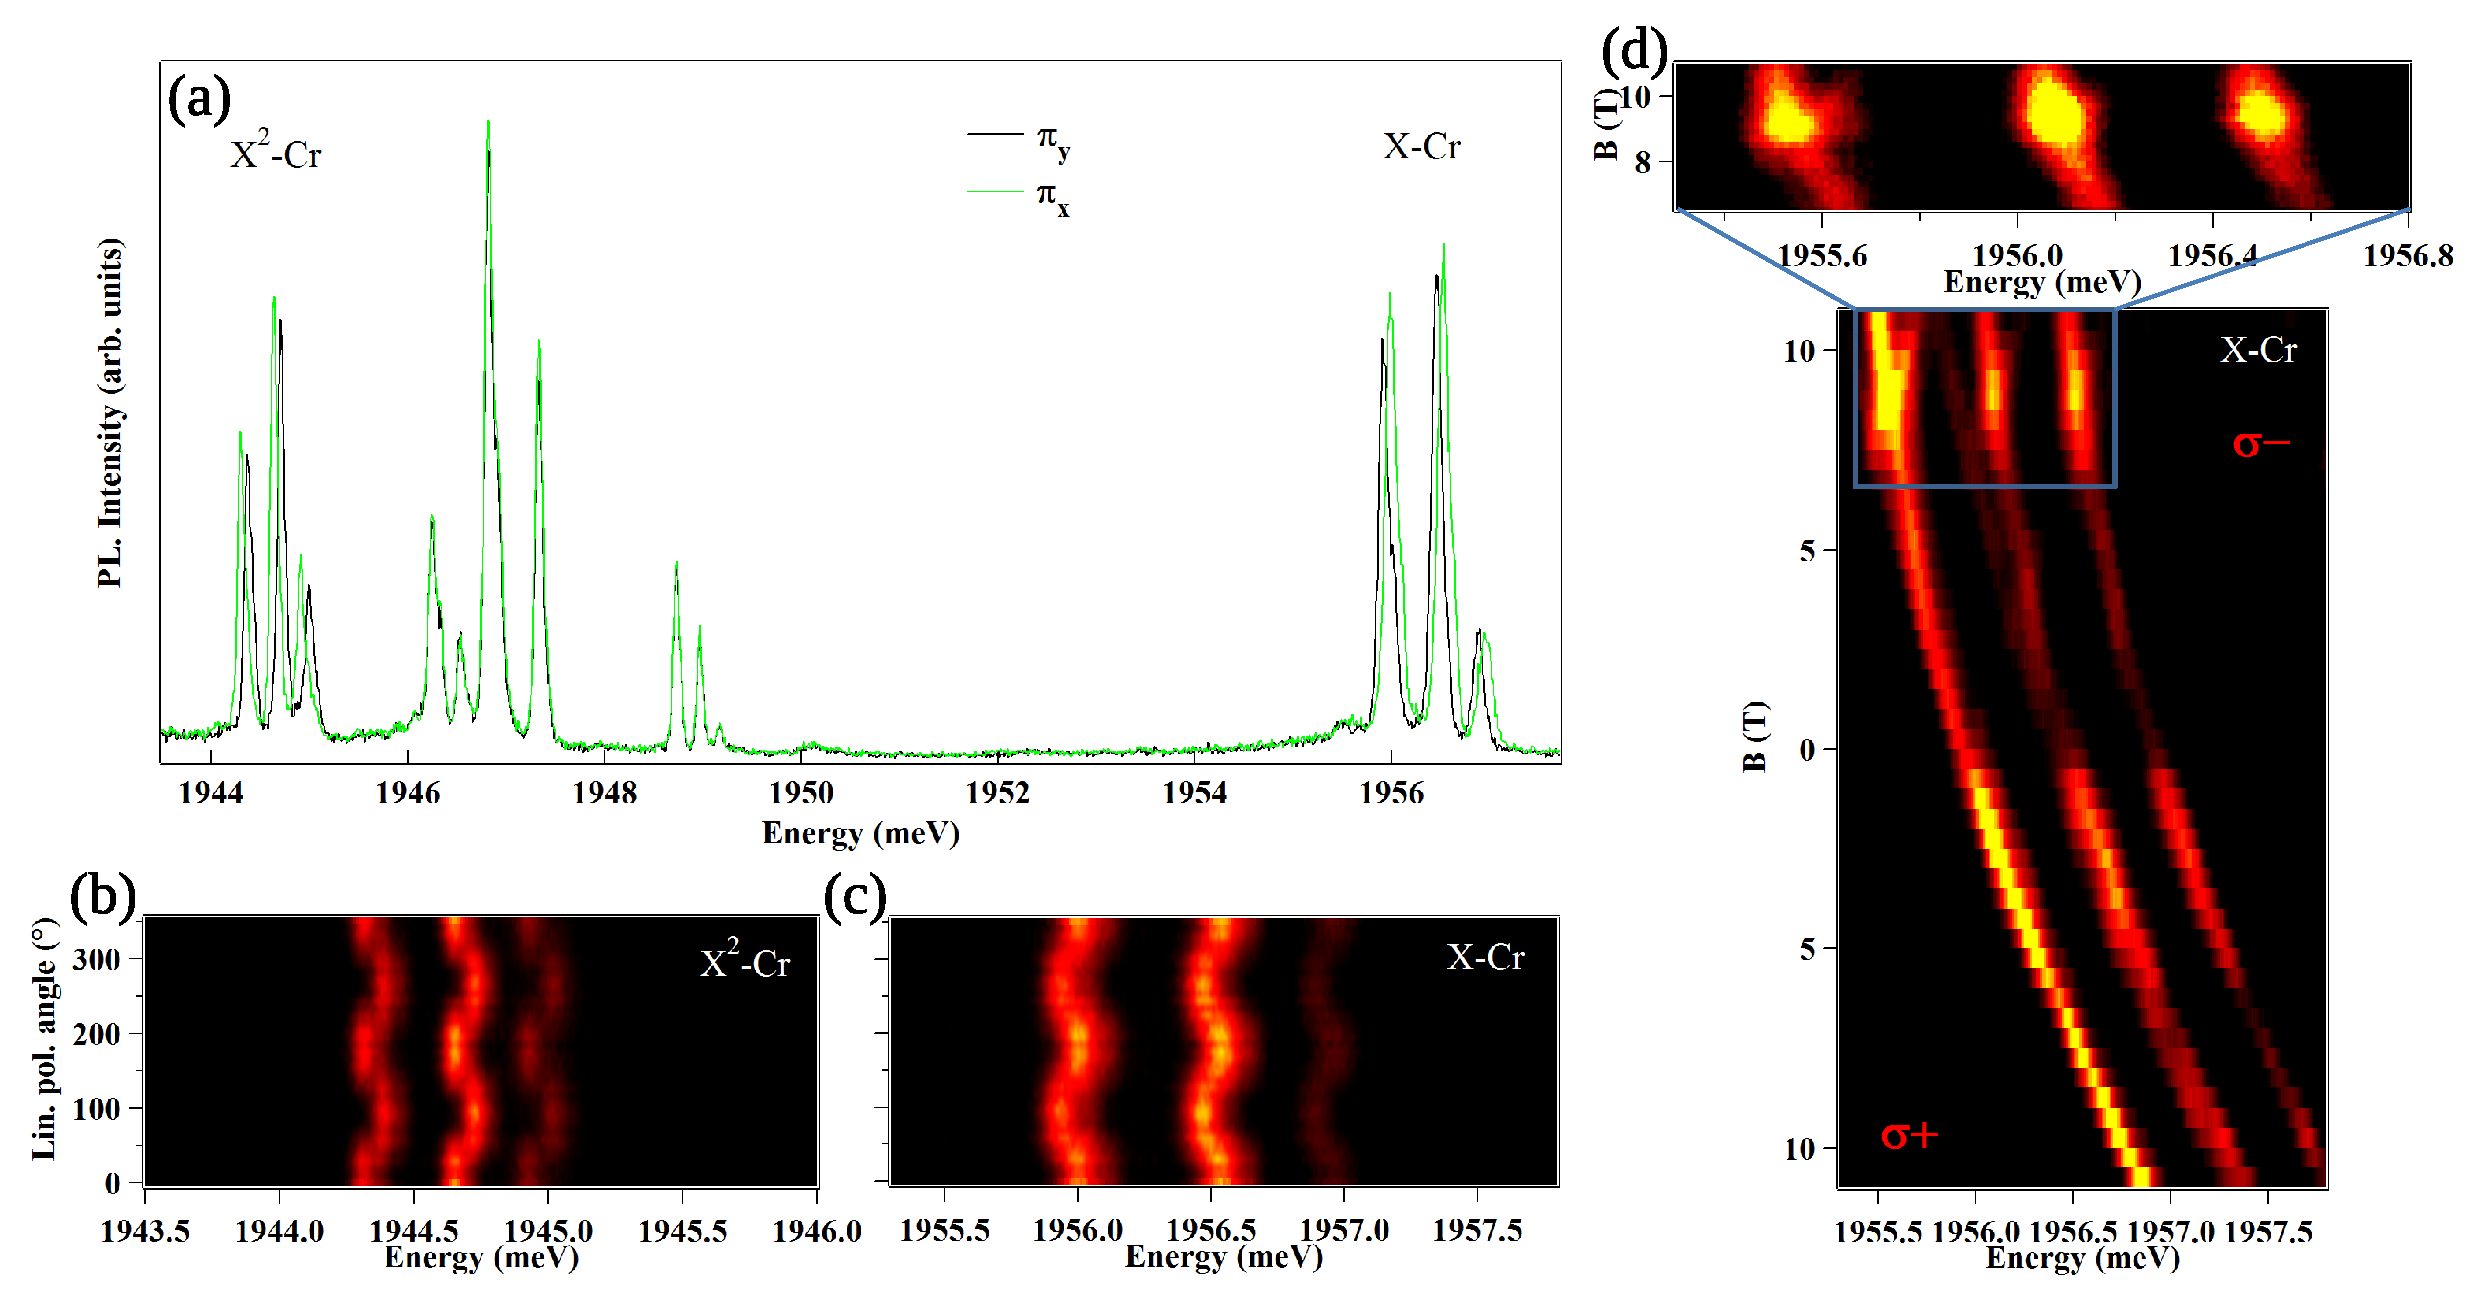
\includegraphics[width=14.9cm]{Pictures/6peaks.eps}
	\end{center}
	\caption{(a) QD5 (found in dot390) linearly polarized low temperature (T = 5 K) PL intensity at zero magnetic field. (b) - (c) Respectively QD5 X$^2$-Cr and X-Cr linear polarization PL dependence at zero magnetic field. (c) X-Cr magnetic field PL dependence of QD5. Zoom on presents anti-crossing appearing at $B_z = 9$ T.}
	\label{CrSixPeaksMagOpt}
	\end{figure}
	
	The evolution under magnetic field of the three peaks differs strongly from the case presented in Sec.~\ref{MagOptCr} and modeled in Sec.~\ref{QDParam}. The same shift is observed on all the lines from $-10$ T to $+10$ T. However, none of the anti-crossings explained before is present. A single anti-crossing appears on all the peaks for B = 9 T in $\sigma-$ polarization. These anti-crossings arise from the mixing between bright and dark exciton, as observed in non-magnetic QDs~\cite{QDFineStruct}. The PL map is similar to the one expected for three non-magnetic QDs emitting at close energies. However, all the peaks were found to have their maximum intensity for the same laser position on the sample surface, and they share the same excited states. It is highly improbable to find three dots close to each other, emitting almost at the same energy and sharing excited states at several position on the sample and many similar dots were found in Cr-doped samples.

	\begin{figure}[h!]
	\begin{center}
		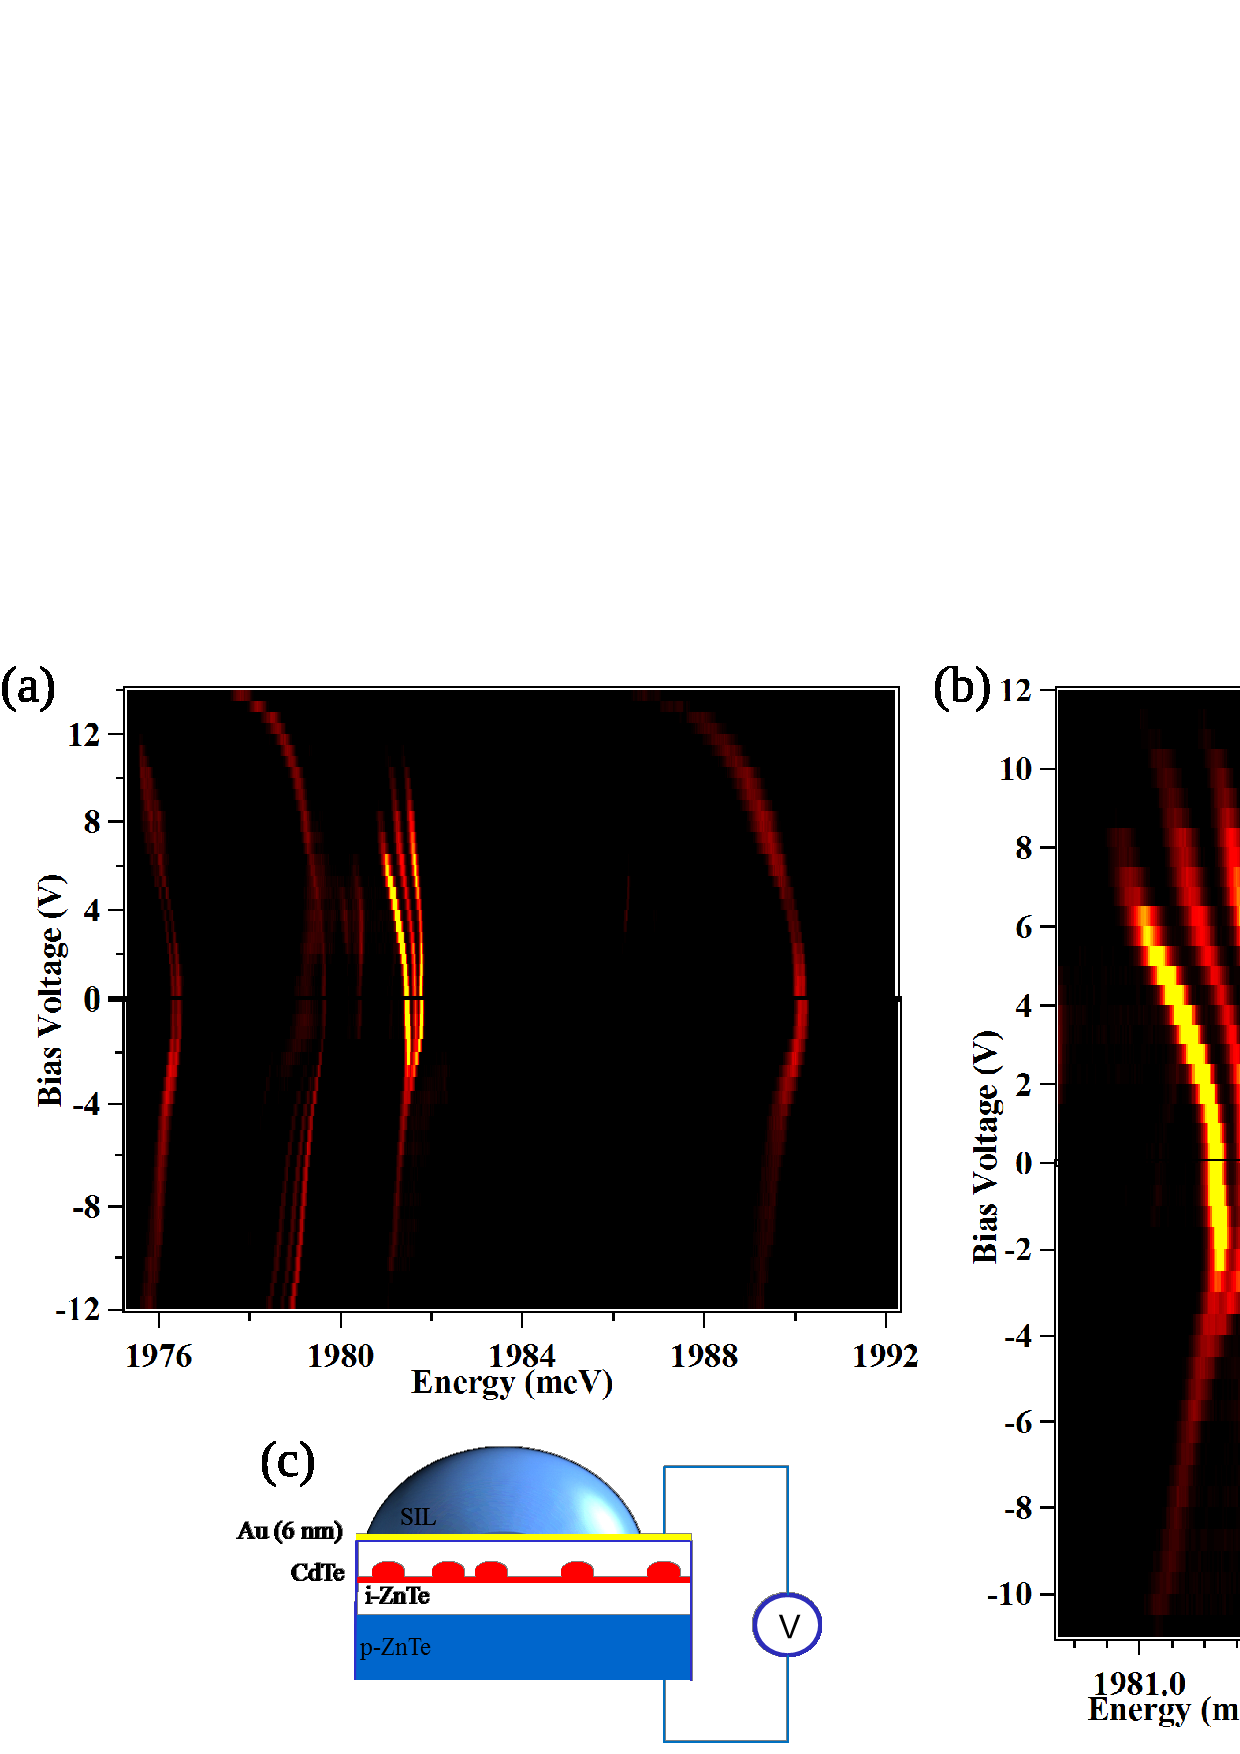
\includegraphics[width=12cm]{Pictures/EfieldX-Xc.png}
	\end{center}
	\caption{(a) QD6 (dot390) PL evolution under application of a bias voltage accross the QD. (b) Zoom on X$^+$-Cr circular polarization PL intensity evolution under electric field. A strong stark shift is observed, as well as variation in the splitting between the lines. (c) Schema of a sample with a Schottky gate used to to control the charge state of the QD. See Sec.~II.3.1%~\ref{ChargedSample}
for more details}
	\label{CrSixPeaksEFieldX+}
	\end{figure}	
	
	To better understand the nature of those dots those dots, the evolution of their emission under bias voltage was studied. The application of an electric field was realized via a Schottky gate deposited on the MBE grown sample as presented in Sec.~II.3.1%~\ref{ChargedSample}
. Fig.~\ref{CrSixPeaksEFieldX+} (a) presents such a PL map versus bias voltage. The first visible feature is the strong electric field dependency of the emission energy, more pronounced for X-Cr than for X$^+$-Cr and X$^-$-Cr. The maximum shift of X-Cr is of about 2.9 meV.
	
	Another remarkable point is evidenced in Fig.~\ref{CrSixPeaksEFieldX+}(b): the splitting between each peak of X$^+$-Cr changes with the applied electric field. The total splitting, measured between the high and low energy peaks, decreases from about 0.7 meV at 8 V down to 0 meV at -4.5 V.
	
	\begin{figure}[h!]
	\begin{center}
		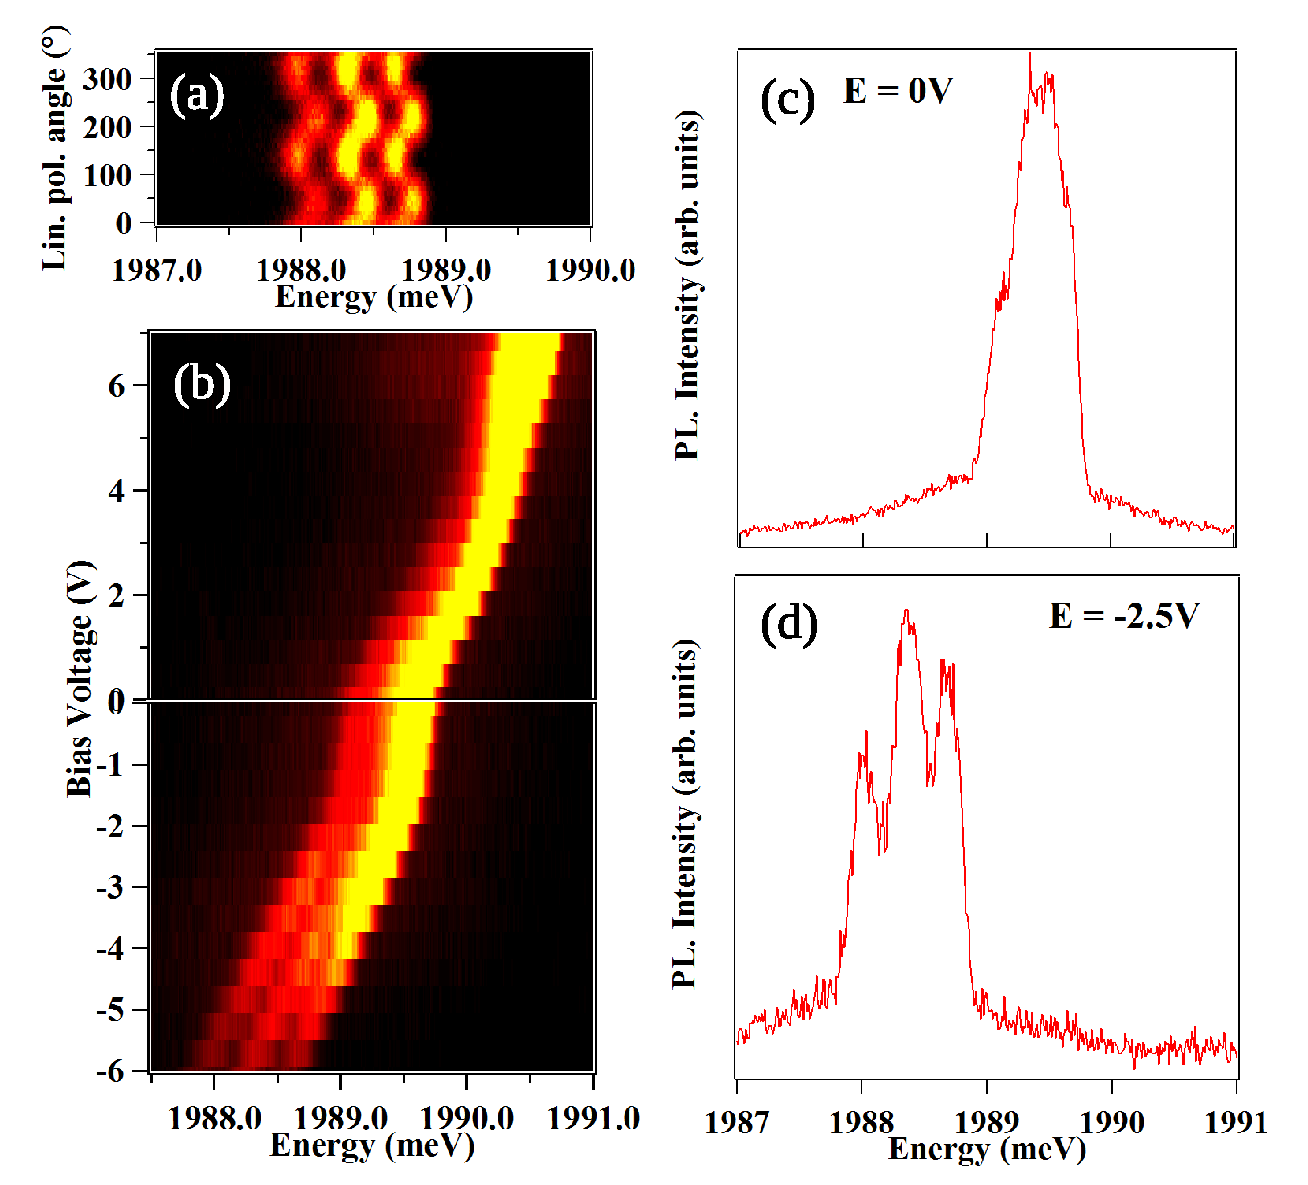
\includegraphics[width=12cm]{Pictures/SplitUnderEfiledXCr.eps}
	\end{center}
	\caption{PL of X-Cr in QD7 (dot390) at $T = 5$ K. (a) Linear polarization dependence of the PL intensity, taken at -2.5V bias voltage. (b) Circular PL intensity evolution as a function of the applied bias voltage. (c)-(d) Circular PL for an applied bias voltage of, respectively, 0V and -2.5V.}
	\label{CrSixPeaksSplit}
	\end{figure}
		
	Fig.~\ref{CrSixPeaksSplit} shows that, using bias voltage, one can manipulate the splitting of any given charged state of the QD. For all positive bias voltages between 0V and 7V, X-Cr presents a broad emission containing six peaks in linear emission, as show on Fig.~\ref{CrSixPeaksSplit}(a). For bias voltage below -1V, the PL divides into three peaks (Fig.~\ref{CrSixPeaksSplit}(d)).
	
	\begin{figure}[h!]
	\begin{center}
		\includegraphics[width=14.9cm]{Pictures/CrCloseDot.png}
	\end{center}
	\caption{(a) Cr accessible charged states in ZnTe~\cite{CrZnTe}. (b)-(d) Illustration of the effect of a punctual charge on the wavefunction of an electron (red) and a hole (yellow) in a quantum dots.}
	\label{CrOutsideDot}
	\end{figure}
	
%	It is possible for the emission of a quantum dot to fluctuate between different energy under fluctuation of charge in the vicinity of a QD. This phenomena leads to a peak broadening~\cite{ChargeSpectFluct} as well as spectrum jumps. For the PL to jump between three emission energies, the charge fluctuation has to be able to take three distinct charge values.
	
	The structure found at $B_z = 0$ T is expected for QDs with a large in-plane anisotropy term $E$, as presented in Sec.~\ref{QDParam}. However, the behaviour of these QDs under magnetic field and application of bias voltage is not consistent with high $E$ QDs.
	
	We propose that the PL behaviour presented in Fig.~\ref{CrSixPeaksMagOpt}, \ref{CrSixPeaksEFieldX+} and \ref{CrSixPeaksSplit} is due to the presence of Cr atoms in the ZnTe barrier close to the dot. As shown on Fig.\ref{CrOutsideDot} (a), the transitions Cr$^+$/Cr$^{2+}$ and Cr$^{2+}$/Cr$^{3+}$ states are in the gap and accessible~\cite{CrZnTe}, either by capturing an electron (Cr$^+$) or a hole (Cr$^{3+}$). Cr$^{2+}$ is the neutral state of Cr in ZnTe, sharing its outer shell electrons to bind with the atoms of the crystal. Capturing an electron, the Cr atom attracts the hole confined in the QD and repel the electron. The opposite happens when the Cr captures a hole. The ion can be viewed as a punctual charge, which effect on the electron and hole wave functions is schematically presented in Fig.\ref{CrOutsideDot}(b)-(d).
	
	The electron is well confined in CdTe/ZnTe quantum dots and is thus not affected strongly by the presence of a punctual charge close to the QD. The hole, on the other hand, is only weakly confined in CdTe/ZnTe QDs. Its wave function is then strongly affected by the charge variations of the Cr sitting in the vicinity of the QD. It is deformed by the ion electric field, being repel when the atom capture a hole, attracted when it capture an electron. This deformation affects the hole-electron interaction, and thus the emission energy of the exciton.
	
	The application of an electric field through the Schottky gate attract the hole toward the surface or the back of the sample, depending on the direction of the applied field. This changes the hole interaction with the Cr ion. For a high bias voltage, the h-Cr Coulomb interaction becomes negligible, and the splitting induced by the variation of teh charge of the ion disappears.

	These variations of a charge close to the dot would also explain the apparent the difference of splitting between the different excitonic complex. The application of a magnetic field change the excitonic species binding energy, changing their emission energy~\cite{BesombesEfieldExciton}. However, each species is affected differently: the shift energy can be smaller, or even, for X$^-$, the shift for a given electric field is opposed to the one of other species. These different shifts of the different excitonic complexes lead to different apparent splittings.
%	This weak confinement also mean that the wavefunction goes slightly out of the dot, and thus the overlap with the Cr atom might exist for the hole, even if the atom is not in the QD. The slight overlap is enough to cause the splitting of the exciton emission PL via the exchange interaction, without the Cr being affected by the dot. When the atom get a positive charge, it will repel the hole, reducing the overlap until none remain, killing the splitting of the emission. The opposite happens when the Cr capture an electron, attracting the hole and improving the overlap. The overlap can also be affected by the application of a magnetic field through the Schottky gate, which will change the  wavefunctions shape and the probability for the Cr atom to be in a given charge state.
%
%	The charge variation of the Cr is of the value of the elementary charge. Considering a pure coulomb interaction between two punctual charges, for a charge at 5nm of the dot, its effect is of the same order of magnitude than the hole-Cr exchange interaction. In order to have a significant effect on the dot PL, the Cr has then to be close to it, not more than a few nanometres away. 
	
	This hypothesis of a Cr in the barrier causing these three peaks emission is currently studied more in details. SIMS and TEM experiments have been proposed to test the possibility for the Cr to diffuse outside the quantum dots layer during the MBE growth. Optically, it has been proposed to excite the Cr$^{2+}$/Cr$^{3+}$ transition using a Near Infrared (NIR) laser: this should change the probability of the Cr to be in the Cr$^{3+}$ configuration, and thus the intensity distribution of the complexes, with the peak associated with Cr$^{3+}$ becoming more intense.
	
	\section*{Conclusion}
	
%	For the first time, a single Cr atom was embedded inside a II-VI quantum dot. We were then able to probe it optically. Such a system presents a characteristic three peak emission, along with the emission of a dark state on the low energy side. The action of the magnetic anisotropy, splitting the Cr spin states according to $D_0 S_z^2$, is strong enough to keep the $S_z = \pm2$ level to be thermally populated, and thus they do not present luminescence. The QDs show a good spin conversation during the exciton lifetime inside the dot, thanks to the effective magnetic field created by the Cr spin. Magneto-optics confirm the chosen energy structure and gives us the possibility to deduce the magnitude of several of the quantum dot parameters. We used the model to simulate the emission of QD with different parameters, and proposed an explanation to the absence of high anisotropy QDs in the one we probed. Some dots seems to correspond to these high anisotropy QDs, but they show no sign of magnetic atom inside them under further investigation. We finished proposing a possible explanation for those dots, supposing the presence of Cr atoms in the ZnTe barrier.
	
	For the first time, the physics of a single Cr atom embedded in a II-VI QD was studied. Its spin was probed optically under magnetic field. The energy structure of the Cr spin in a self-assembled QD was deduced from this experiment. It evidenced that the splitting caused by the magnetic anisotropy is strong enough to keep the states $S_z = \pm2$ to be thermally populated. Several anti-crossing characteristic from a Cr-doped QDs appears under magnetic field, opening the possibility to extract parameters of the dot. The evolution of the PL under magnetic field also evidence that the h-Cr coupling is anti-ferromagnetic, contrary to what was suggested in the literature. 
	
	Having successfully inserted and probed single Cr atom spins in CdTe/ZnTe quantum dots, it is now important to study how this system evolves in time. An important step for further use of the Cr as an hybrid spin-mechanical system is the possibility to prepare the Cr spin in a chosen state, and then control it.

\printbibliography

\end{document}
